\chapter{Điện từ trường tương đối tính}


\begin{vd}[Hạt chuyển động trong điện trường và từ trường]
Bài toán này nghiên cứu chuyển động của các hạt trong điện trường và từ trường trong điều kiện không trọng lực.
\begin{enumerate}[1)]
    \item Ở giữa hai bản tụ phẳng và song song, đặt cách nhau một khoảng $d$ của một tụ điện, người ta tạo ra một điện trường đều bằng cách kết nối các bản tụ điện với một điện áp không đổi ${U}$. Đồng thời, trong khoảng không gian giữa hai bản tụ điện, người ta tạo ra một từ trường đều có cảm ứng $\ot{B}$ và các đường sức từ vuông góc với các đường sức điện. Một electron tự do khối lượng ${m}$ và độ lớn điện tích $e$ được đưa vào sát bản tụ điện âm.
    \begin{enumerate}[a)]
        \item Xác định biểu thức các thành phần vận tốc $\left(v_{x}, v_{y}, v_{z}\right)$ của electron như một hàm của thời gian và các hằng số đã cho trong đề bài.
        \item Hãy biểu diễn các thành phần vận tốc electron như hàm của tọa độ $y$ (song song với đường sức điện trường): $v_{x} = v_{x}(y)$ và $v_{y} = v_{y}(y)$.
    \end{enumerate}
    \item Để xác định các tính chất của một chùm hạt tương đối tính mang điện dương $e$, người ta cho chùm tia đi qua một vùng từ trường đều $\ot{B}$ (hình $a$). Cho một chùm hạt giống y như hình $a$ đi qua một vùng điện trường đều $\ot{E}$ (hình $b$). Từ trường và điện trường làm lệch đường đi của các chùm hạt các góc nhỏ $\alpha_{B}$ và $\alpha_{E}, ~\left(\alpha_{B} \ll 1, \alpha_{E} \ll 1\right)$. Hai khu vực có từ trường và điện trường đều có chiều rộng $\ell$.
       \begin{center}
\tikzset{every picture/.style={line width=0.75pt}} %set default line width to 0.75pt        

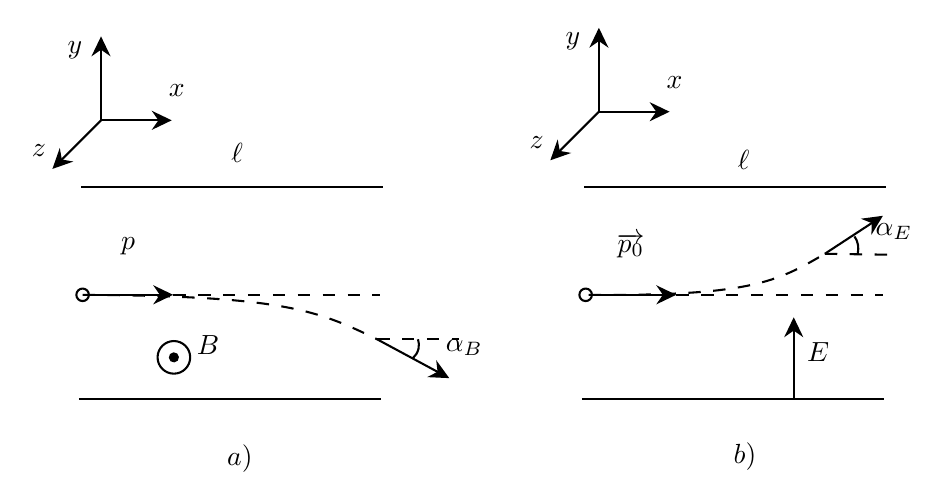
\begin{tikzpicture}[x=0.75pt,y=0.75pt,yscale=-0.9,xscale=0.9]
%uncomment if require: \path (0,469); %set diagram left start at 0, and has height of 469

%Straight Lines [id:da4837992507155702] 
\draw    (116.97,145.52) -- (278.57,145.52) ;
%Straight Lines [id:da3618373284849863] 
\draw    (115.78,259.04) -- (277.38,259.04) ;
%Straight Lines [id:da9125907838825991] 
\draw    (120.1,203.46) -- (163.23,203.46) ;
\draw [shift={(166.23,203.46)}, rotate = 180] [fill={rgb, 255:red, 0; green, 0; blue, 0 }  ][line width=0.08]  [draw opacity=0] (10.72,-5.15) -- (0,0) -- (10.72,5.15) -- (7.12,0) -- cycle    ;
\draw [shift={(117.75,203.46)}, rotate = 0] [color={rgb, 255:red, 0; green, 0; blue, 0 }  ][line width=0.75]      (0, 0) circle [x radius= 3.35, y radius= 3.35]   ;
%Shape: Ellipse [id:dp7481755649873225] 
\draw   (157.88,236.93) .. controls (157.88,232.11) and (161.79,228.2) .. (166.61,228.2) .. controls (171.43,228.2) and (175.34,232.11) .. (175.34,236.93) .. controls (175.34,241.76) and (171.43,245.67) .. (166.61,245.67) .. controls (161.79,245.67) and (157.88,241.76) .. (157.88,236.93) -- cycle ;
%Shape: Ellipse [id:dp3186635906667177] 
\draw  [fill={rgb, 255:red, 0; green, 0; blue, 0 }  ,fill opacity=1 ] (164.5,237.1) .. controls (164.4,235.94) and (165.27,234.91) .. (166.44,234.82) .. controls (167.61,234.73) and (168.63,235.6) .. (168.72,236.76) .. controls (168.82,237.93) and (167.95,238.95) .. (166.78,239.05) .. controls (165.61,239.14) and (164.59,238.27) .. (164.5,237.1) -- cycle ;
%Straight Lines [id:da6893112371800201] 
\draw  [dash pattern={on 4.5pt off 4.5pt}]  (166.23,203.46) -- (276.83,203.46) ;
%Curve Lines [id:da8515306495177755] 
\draw  [dash pattern={on 4.5pt off 4.5pt}]  (117.75,203.46) .. controls (225.28,204.09) and (243.25,211.66) .. (275.41,227.27) ;
%Straight Lines [id:da4446918819851766] 
\draw    (275.41,227.27) -- (311.4,246.64) ;
\draw [shift={(314.04,248.06)}, rotate = 208.29] [fill={rgb, 255:red, 0; green, 0; blue, 0 }  ][line width=0.08]  [draw opacity=0] (10.72,-5.15) -- (0,0) -- (10.72,5.15) -- (7.12,0) -- cycle    ;
%Straight Lines [id:da9893316794667517] 
\draw    (127.61,110.05) -- (127.61,68.12) ;
\draw [shift={(127.61,65.12)}, rotate = 450] [fill={rgb, 255:red, 0; green, 0; blue, 0 }  ][line width=0.08]  [draw opacity=0] (10.72,-5.15) -- (0,0) -- (10.72,5.15) -- (7.12,0) -- cycle    ;
%Straight Lines [id:da8283494203137156] 
\draw    (127.61,110.05) -- (162.45,110.05) ;
\draw [shift={(165.45,110.05)}, rotate = 180] [fill={rgb, 255:red, 0; green, 0; blue, 0 }  ][line width=0.08]  [draw opacity=0] (10.72,-5.15) -- (0,0) -- (10.72,5.15) -- (7.12,0) -- cycle    ;
%Straight Lines [id:da01804388756794495] 
\draw    (127.61,110.05) -- (103.72,133.94) ;
\draw [shift={(101.59,136.06)}, rotate = 315] [fill={rgb, 255:red, 0; green, 0; blue, 0 }  ][line width=0.08]  [draw opacity=0] (10.72,-5.15) -- (0,0) -- (10.72,5.15) -- (7.12,0) -- cycle    ;
%Straight Lines [id:da43158252166059596] 
\draw  [dash pattern={on 4.5pt off 4.5pt}]  (275.41,227.27) -- (319.16,227.27) ;
%Shape: Arc [id:dp9665131325952021] 
\draw  [draw opacity=0] (297.29,227.27) .. controls (297.84,228.86) and (297.96,230.61) .. (297.56,232.36) .. controls (297.1,234.39) and (296.01,236.1) .. (294.54,237.36) -- (288.5,230.29) -- cycle ; \draw   (297.29,227.27) .. controls (297.84,228.86) and (297.96,230.61) .. (297.56,232.36) .. controls (297.1,234.39) and (296.01,236.1) .. (294.54,237.36) ;
%Straight Lines [id:da19159802170881934] 
\draw    (386.26,145.52) -- (547.86,145.52) ;
%Straight Lines [id:da8358521727332122] 
\draw    (385.08,259.04) -- (546.68,259.04) ;
%Straight Lines [id:da5574462908594422] 
\draw    (389.4,203.46) -- (432.53,203.46) ;
\draw [shift={(435.53,203.46)}, rotate = 180] [fill={rgb, 255:red, 0; green, 0; blue, 0 }  ][line width=0.08]  [draw opacity=0] (10.72,-5.15) -- (0,0) -- (10.72,5.15) -- (7.12,0) -- cycle    ;
\draw [shift={(387.05,203.46)}, rotate = 0] [color={rgb, 255:red, 0; green, 0; blue, 0 }  ][line width=0.75]      (0, 0) circle [x radius= 3.35, y radius= 3.35]   ;
%Straight Lines [id:da39592654389589965] 
\draw  [dash pattern={on 4.5pt off 4.5pt}]  (435.53,203.46) -- (546.13,203.46) ;
%Curve Lines [id:da09246772294266825] 
\draw  [dash pattern={on 4.5pt off 4.5pt}]  (388.69,203.49) .. controls (474.73,204.1) and (489.19,196.74) .. (515.07,181.5) ;
%Straight Lines [id:da4406856308350531] 
\draw    (515.07,181.5) -- (543.66,162.8) ;
\draw [shift={(546.17,161.16)}, rotate = 506.81] [fill={rgb, 255:red, 0; green, 0; blue, 0 }  ][line width=0.08]  [draw opacity=0] (10.72,-5.15) -- (0,0) -- (10.72,5.15) -- (7.12,0) -- cycle    ;
%Straight Lines [id:da521869820163753] 
\draw  [dash pattern={on 4.5pt off 4.5pt}]  (515.07,181.5) -- (550.07,182) ;
%Shape: Arc [id:dp32176011030124063] 
\draw  [draw opacity=0] (532.76,181) .. controls (533.05,179.63) and (533.09,178.15) .. (532.83,176.66) .. controls (532.54,174.93) and (531.87,173.42) .. (530.96,172.22) -- (525.56,178.63) -- cycle ; \draw   (532.76,181) .. controls (533.05,179.63) and (533.09,178.15) .. (532.83,176.66) .. controls (532.54,174.93) and (531.87,173.42) .. (530.96,172.22) ;
%Straight Lines [id:da32259941560536354] 
\draw    (498.44,259.19) -- (498.44,218.49) ;
\draw [shift={(498.44,215.49)}, rotate = 450] [fill={rgb, 255:red, 0; green, 0; blue, 0 }  ][line width=0.08]  [draw opacity=0] (10.72,-5.15) -- (0,0) -- (10.72,5.15) -- (7.12,0) -- cycle    ;
%Straight Lines [id:da25563058133965644] 
\draw    (394.14,105.44) -- (394.14,63.51) ;
\draw [shift={(394.14,60.51)}, rotate = 450] [fill={rgb, 255:red, 0; green, 0; blue, 0 }  ][line width=0.08]  [draw opacity=0] (10.72,-5.15) -- (0,0) -- (10.72,5.15) -- (7.12,0) -- cycle    ;
%Straight Lines [id:da8030711351743123] 
\draw    (394.14,105.44) -- (428.98,105.44) ;
\draw [shift={(431.98,105.44)}, rotate = 180] [fill={rgb, 255:red, 0; green, 0; blue, 0 }  ][line width=0.08]  [draw opacity=0] (10.72,-5.15) -- (0,0) -- (10.72,5.15) -- (7.12,0) -- cycle    ;
%Straight Lines [id:da7043971087333081] 
\draw    (394.14,105.44) -- (370.25,129.33) ;
\draw [shift={(368.13,131.45)}, rotate = 315] [fill={rgb, 255:red, 0; green, 0; blue, 0 }  ][line width=0.08]  [draw opacity=0] (10.72,-5.15) -- (0,0) -- (10.72,5.15) -- (7.12,0) -- cycle    ;

% Text Node
\draw (136.74,171.01) node [anchor=north west][inner sep=0.75pt]    {$\ot{p}$};
% Text Node
\draw (177.26,223.49) node [anchor=north west][inner sep=0.75pt]    {$\ot{B}$};
% Text Node
\draw (195.68,120.85) node [anchor=north west][inner sep=0.75pt]    {$\ell $};
% Text Node
\draw (162.21,89.33) node [anchor=north west][inner sep=0.75pt]    {$x$};
% Text Node
\draw (108.08,66.06) node [anchor=north west][inner sep=0.75pt]    {$y$};
% Text Node
\draw (88.9,121.51) node [anchor=north west][inner sep=0.75pt]    {$z$};
% Text Node
\draw (310.56,225.61) node [anchor=north west][inner sep=0.75pt]    {$\alpha_{B}$};
% Text Node
\draw (402.16,168.93) node [anchor=north west][inner sep=0.75pt]    {$\overrightarrow{p_{0}}$};
% Text Node
\draw (466.82,124.54) node [anchor=north west][inner sep=0.75pt]    {$\ell $};
% Text Node
\draw (540.59,163.62) node [anchor=north west][inner sep=0.75pt]    {$\alpha_{E}$};
% Text Node
\draw (503.97,227.41) node [anchor=north west][inner sep=0.75pt]    {$\ot{E}$};
% Text Node
\draw (193.51,282.03) node [anchor=north west][inner sep=0.75pt]    {$a)$};
% Text Node
\draw (464.65,281.1) node [anchor=north west][inner sep=0.75pt]    {$b)$};
% Text Node
\draw (428.74,84.71) node [anchor=north west][inner sep=0.75pt]    {$x$};
% Text Node
\draw (374.61,61.44) node [anchor=north west][inner sep=0.75pt]    {$y$};
% Text Node
\draw (355.43,116.9) node [anchor=north west][inner sep=0.75pt]    {$z$};
\end{tikzpicture}

    \end{center}
    \begin{enumerate}[a)]
        \item Xác định động lượng của hạt $p$ trước khi nó bay vào vùng từ trường.
        \item Gọi động lượng của hạt trước khi vào điện trường là $p_0$, hãy biểu diễn năng lượng ban đầu $W_0$ của hạt theo độ lệch theo phương $y$ (và cả $\alpha_E$) sau khi nó ra khỏi vùng điện trường.
    \end{enumerate}
\end{enumerate}
\end{vd}
\begin{loigiai}
\begin{enumerate}[1)]
    \item 
    \begin{enumerate}[a)]
        \item Chọn chiều dương như hình vẽ.
        \begin{center}


\tikzset{every picture/.style={line width=0.75pt}} %set default line width to 0.75pt        

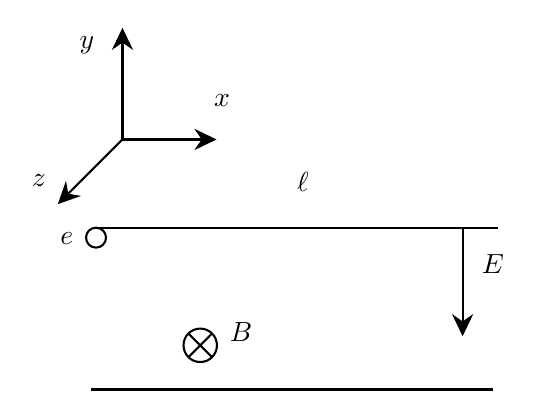
\begin{tikzpicture}[x=0.75pt,y=0.75pt,yscale=-1,xscale=1]
%uncomment if require: \path (0,400); %set diagram left start at 0, and has height of 400

%Straight Lines [id:da18177163048545708] 
\draw    (209.71,170.71) -- (403.26,170.71) ;
%Straight Lines [id:da8800539895479706] 
\draw    (207.3,248.67) -- (400.85,248.67) ;
%Straight Lines [id:da5935461854992317] 
\draw    (222.46,128.22) -- (222.46,77.41) ;
\draw [shift={(222.46,74.41)}, rotate = 450] [fill={rgb, 255:red, 0; green, 0; blue, 0 }  ][line width=0.08]  [draw opacity=0] (10.72,-5.15) -- (0,0) -- (10.72,5.15) -- (7.12,0) -- cycle    ;
%Straight Lines [id:da3808209988082294] 
\draw    (222.46,128.22) -- (264.78,128.22) ;
\draw [shift={(267.78,128.22)}, rotate = 180] [fill={rgb, 255:red, 0; green, 0; blue, 0 }  ][line width=0.08]  [draw opacity=0] (10.72,-5.15) -- (0,0) -- (10.72,5.15) -- (7.12,0) -- cycle    ;
%Straight Lines [id:da3300282521869966] 
\draw    (222.46,128.22) -- (193.42,157.26) ;
\draw [shift={(191.3,159.38)}, rotate = 315] [fill={rgb, 255:red, 0; green, 0; blue, 0 }  ][line width=0.08]  [draw opacity=0] (10.72,-5.15) -- (0,0) -- (10.72,5.15) -- (7.12,0) -- cycle    ;
%Flowchart: Summing Junction [id:dp9962429153507433] 
\draw   (251.87,227.39) .. controls (251.87,222.94) and (255.48,219.33) .. (259.93,219.33) .. controls (264.38,219.33) and (267.98,222.94) .. (267.98,227.39) .. controls (267.98,231.84) and (264.38,235.45) .. (259.93,235.45) .. controls (255.48,235.45) and (251.87,231.84) .. (251.87,227.39) -- cycle ; \draw   (254.23,221.69) -- (265.62,233.09) ; \draw   (265.62,221.69) -- (254.23,233.09) ;
%Straight Lines [id:da11218789827321074] 
\draw    (386.34,220.01) -- (386.34,170.67) ;
\draw [shift={(386.34,223.01)}, rotate = 270] [fill={rgb, 255:red, 0; green, 0; blue, 0 }  ][line width=0.08]  [draw opacity=0] (10.72,-5.15) -- (0,0) -- (10.72,5.15) -- (7.12,0) -- cycle    ;
%Shape: Circle [id:dp24580327405298807] 
\draw   (204.9,175.52) .. controls (204.9,172.86) and (207.05,170.71) .. (209.71,170.71) .. controls (212.37,170.71) and (214.52,172.86) .. (214.52,175.52) .. controls (214.52,178.18) and (212.37,180.33) .. (209.71,180.33) .. controls (207.05,180.33) and (204.9,178.18) .. (204.9,175.52) -- cycle ;

% Text Node
\draw (272.7,214.99) node [anchor=north west][inner sep=0.75pt]    {$\ot{B}$};
% Text Node
\draw (305.17,142.66) node [anchor=north west][inner sep=0.75pt]    {$\ell $};
% Text Node
\draw (265.09,104.9) node [anchor=north west][inner sep=0.75pt]    {$x$};
% Text Node
\draw (200.26,77.03) node [anchor=north west][inner sep=0.75pt]    {$y$};
% Text Node
\draw (177.29,143.45) node [anchor=north west][inner sep=0.75pt]    {$z$};
% Text Node
\draw (394.15,182.25) node [anchor=north west][inner sep=0.75pt]    {$\ot{E}$};
% Text Node
\draw (191,171.73) node [anchor=north west][inner sep=0.75pt]    {$e$};
\end{tikzpicture}
        \end{center}
        Áp dụng định luật II Newton:
\[m\overrightarrow{a} = -e\overrightarrow{E} - e\left(\overrightarrow{v}\times\overrightarrow{B}\right).\]
Chiếu lên các trục tọa độ, ta được
\[\heva{m{{a}_{x}} &= e{{v}_{y}}B,  \\
   m{{a}_{y}} &= eE - e{{v}_{x}}B,  \\
   m{{a}_{z}} &= 0. } \] 

Từ đây, ta biến đổi được 
\[\heva{v_x' &= \dfrac{eB}{m}v_y, \\ {{v}_{x}} &= \dfrac{E}{B}-\frac{m}{eB}{{a}_{y}} \rt v_x' = -\dfrac{m}{eB}v_y'', \\ v_z &= \mathrm{const} = 0. } \tag{1}\label{q.st.1.1}\]
Suy ra
\[v_y'' + \tron{\dfrac{eB}{m}}^2 v_y = 0.\]
Nghiệm của phương trình này có dạng
\[{{v}_{y}} = A\cos \tron{\omega t+\varphi } \quad \text{với}\quad \omega = \dfrac{eB}{m}. \]
Tại $t = 0$, $\heva{v_x &= v_y = v_z = 0,\\ a_y &= \dfrac{eE}{m}} \rt \heva{A\cos \varphi &= 0, \\- A \omega \sin \varphi &= \dfrac{eE}{m}} \rt \heva{\varphi &= -\dfrac{\pi}{2}, \\ A &= \dfrac{E}{B}.}$ \\
Thay vào phương trình trên, ta được
\[v_y = \dfrac{E}{B} \cos \tron{\omega t - \dfrac{\pi}{2}}  = \dfrac{U}{Bd} \sin \dfrac{eB}{m} t. \tag{2}\label{q.st.1.2}\]
Đạo hàm ta thu được gia tốc theo phương $y$
\[ a_y = v_y' = \dfrac{eE}{m} \cos \dfrac{eB}{m} t. \]
Kết hợp với (\ref{q.st.1.1}), ta suy ra
\[v_x = \dfrac{U}{Bd}\tron{1 - \cos \dfrac{eB}{m} t }.\]
Vậy các thành phần vận tốc của electron 
\[(v_x, v_y, v_z) = \tron{\dfrac{U}{Bd}\tron{1 - \cos \dfrac{eB}{m} t }, \dfrac{U}{Bd} \sin \dfrac{eB}{m} t , 0}. \tag{3}\label{q.st.1.3}\]

    \item  Ta có
    \[y = \int_0^t v_y \dd t =  \dfrac{mU}{ed{{B}^{2}}} \tron{1 - \cos \dfrac{eB}{m} t}.\]
Từ (\ref{q.st.1.3}), suy ra
\[{{v}_{x}}=\dfrac{eB}{m}y.  \]
Áp dụng định luật bảo toàn năng lượng \[\dfrac{m}{2}(v_{x}^{2} + v_{y}^{2}) = {eE}y \Rightarrow {{v}_{y}} = \sqrt{\dfrac{2eU}{md}y - \dfrac{e^2B^2}{m^2} y^2}.\]
    \end{enumerate}
    \item \begin{enumerate}[a)]
        \item Áp dụng định luật II Newton cho chùm hạt tương đối tính
        \[e\left(\overrightarrow{v}\times \overrightarrow{B}\right) = \dfrac{\dd\tron{m\overrightarrow{v}}}{\dd t} = \dfrac{\dd }{\dd t}\tron{\dfrac{{{m}_{0}}}{\sqrt{1 - {{\dfrac{v^2}{c^2}}}}}\overrightarrow v},\]
    vì khi chuyển động trong từ trường độ lớn $v$ không đổi nên $m$ không đổi, do đó
\[e\left(\overrightarrow{v}\times \overrightarrow{B}\right) = \dfrac{\dfrac{{{m}_{0}}}{\sqrt{1-{{\dfrac{v^2}{c^2}}}}}\dd\overrightarrow{v}}{\dd t}=\dfrac{m \dd\overrightarrow{v}}{\dd t} \tag{4}\label{q.st.1.4}.\]
Khi đó ta chiếu (\ref{q.st.1.4}) lên các trục ta được:

\[\heva{m\dfrac{\dd {{v}_{x}}}{\dd t} &= e{{v}_{y}}B,\\  m\dfrac{\dd {{v}_{y}}}{\dd t} &= -e{{v}_{x}}B.} \tag{5}\label{q.st.1.5}\]
Suy ra 
\[v_x'' + \tron{\dfrac{eB}{m}}^2 v_x = 0.\]
Nghiệm của phương trình trên có dạng 
\[{{v}_{x}} = A \cos \tron{\dfrac{eB}{m}t + \varphi}.\]
Tại thời điểm $t = 0$, $\heva{v_x &= \dfrac{p}{m},\\ a_x &= 0} \rt \heva{\varphi &= 0, \\ A &= \dfrac{p}{m}}$. Thay vào phương trình trên
\[v_x = \dfrac{p}{m} \cos \dfrac{eB}{m}t. \tag{6}\label{q.st.1.6}\]
Tích phân lên ta được  
\[x = \dfrac{p}{eB}\sin \dfrac{eB}{m}t.\]	
Thay (\ref{q.st.1.6}) vào (\ref{q.st.1.5}) ta được 
\[{{v}_{y}} = -\dfrac{p}{m}\sin \dfrac{eB}{m}t.\] 	
Tích phân hai vế, ta được
\[y = \dfrac{p}{eB}\cos\dfrac{eB}{m}t.\]
Vậy bán kính quỹ đạo tròn \[R=\sqrt{{{x}^{2}}+{{y}^{2}}}=\dfrac{p}{eB}.\]
Với góc nhỏ, ta có 
\[{{\alpha}_{B}}\approx \dfrac{v_y}{v_x} = \dfrac{\ell}{R}\rt  p = \dfrac{eB\ell}{{{\alpha}_{B}}}.\]
    \item Áp dụng định luật II Newton cho chùm hạt tương đối tính
    \[e\overrightarrow{E} = \dfrac{\dd(m\overrightarrow{v})}{\dd t} = \dfrac{\dd }{\dd t}\tron{\dfrac{{{m}_{0}}}{\sqrt{1-{{\dfrac{v^2}{c^2}}}}}\overrightarrow{v}}. \tag{7}\label{q.st.1.7}\]
Áp dụng định luật bảo toàn năng lượng:
\[W = W_0 + eEy.  \tag{8}\label{q.st.1.8}\] 	
Tại thời điểm $t=0$, \[{W}_{0}^{2}={{({{m}_{0}}{{c}^{2}})}^{2}}+{{({{p}_{0}}c)}^{2}}.\tag{9}\label{q.st.1.9}\]  
Tại thời điểm $t$, 
\[{{{W}}^{2}}={{({{m}_{0}}{{c}^{2}})}^{2}}+{{(pc)}^{2}}. \tag{10}\label{q.st.1.10}\] 		
Mặt khác ta lại có 
\[ p = \sqrt{p_{x}^{2} + p_{y}^{2}} = \sqrt{p_{0}^{2} + p_{y}^{2}}.\tag{11}\label{q.st.1.11}\]		
Và vì góc nhỏ nên 
\[{{\alpha}_{E}}\approx \tan {{\alpha }_{E}} = \dfrac{{{p}_{y}}}{{{p}_{x}}} = \dfrac{{{p}_{y}}}{{{p}_{0}}}\rt {{p}_{y}} = {{p}_{0}}{{\alpha }_{E}}. \tag{12}\label{q.st.1.12}\]
Từ (\ref{q.st.1.9}), (\ref{q.st.1.10}) và (\ref{q.st.1.11}) suy ra 
\[{{{W}}^{2}}-{W}_{0}^{2}={{(pc)}^{2}} - {{({{p}_{0}}c)}^{2}}={{c}^{2}}\left[ (p_{0}^{2}+p_{y}^{2})-p_{0}^{2} \right] = p_{y}^{2}{{c}^{2}}.\]
Kết hợp với (\ref{q.st.1.8}) và (\ref{q.st.1.12}) ta được
\[{{({W_{0}}{+eE}y)}^{2}} - {W}_{0}^{2} = \alpha _{E}^{2}p_{0}^{2}{{c}^{2}}\rt {{{W}}_{0}} = \dfrac{\alpha _{E}^{2}p_{0}^{2}{{c}^{2}}{-(eE}y)^{2}}{2eEy}.\]

    \end{enumerate}
\end{enumerate}
\end{loigiai}


\begin{vd}[Chuyển động của proton ở gần một dây dẫn mang dòng điện]
Như hình bên dưới, một proton mang điện tích $+e$ chuyển động với vận tốc $v$ song song với một sợi dây dài, mảnh, ở khoảng cách $r$ tính từ trục của sợi dây. Dây mang dòng điện với cường độ $I$, và điện tích trên mỗi đơn vị dài là $\lambda$ (giả sử là dương và đồng nhất). Cả proton và sợi dây được đặt trong chân không. Viết các câu trả lời từ $1)$ đến $3)$ theo $r$, $I$, $\lambda$ và hằng số độ điện thẩm chân không $\varepsilon_0$, độ từ thẩm $\mu_0$, tốc độ ánh sáng $c$ và các vector đơn vị trong hệ tọa độ trụ $\ot{e_{r}}$, $\ot{e_{\theta}}$, $\ot{e_{z}}$.
\begin{enumerate}[1)]
    \item Tìm điện trường $E$ tại điểm đặt proton.
    \item Tìm từ trường $B$ tại điểm đặt proton.
    \item Tìm tốc độ của proton sao cho nó chuyển động theo một đường thẳng song song với dây dẫn.
\end{enumerate}
\begin{center}
% Gradient Info
\tikzset {_33lxuwqht/.code = {\pgfsetadditionalshadetransform{ \pgftransformshift{\pgfpoint{89.1 bp } { -108.9 bp }  }  \pgftransformscale{1.32 }  }}}
\pgfdeclareradialshading{_3sp9wiugx}{\pgfpoint{-72bp}{88bp}}{rgb(0bp)=(1,1,1);
rgb(0bp)=(1,1,1);
rgb(25bp)=(0,0,0);
rgb(400bp)=(0,0,0)}
\tikzset{every picture/.style={line width=0.75pt}} %set default line width to 0.75pt        

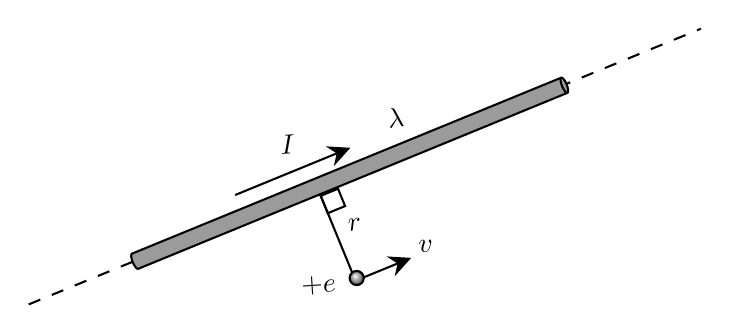
\begin{tikzpicture}[x=0.75pt,y=0.75pt,yscale=-1,xscale=1]
%uncomment if require: \path (0,300); %set diagram left start at 0, and has height of 300

%Straight Lines [id:da7042147037448914] 
\draw  [dash pattern={on 4.5pt off 4.5pt}]  (107.97,178.42) -- (431.81,45.6) ;
%Shape: Can [id:dp496632324424388] 
\draw  [fill={rgb, 255:red, 155; green, 155; blue, 155 }  ,fill opacity=1 ] (367.54,76.5) -- (160.69,161.29) .. controls (160.09,161.54) and (158.93,160.1) .. (158.1,158.09) .. controls (157.28,156.07) and (157.1,154.23) .. (157.7,153.99) -- (364.55,69.19) .. controls (365.15,68.95) and (366.31,70.38) .. (367.14,72.4) .. controls (367.96,74.41) and (368.14,76.25) .. (367.54,76.5) .. controls (366.93,76.74) and (365.77,75.31) .. (364.95,73.29) .. controls (364.12,71.28) and (363.94,69.44) .. (364.55,69.19) ;
%Straight Lines [id:da9711125139120911] 
\draw    (207.43,125.73) -- (260.17,104.11) ;
\draw [shift={(262.95,102.97)}, rotate = 517.7] [fill={rgb, 255:red, 0; green, 0; blue, 0 }  ][line width=0.08]  [draw opacity=0] (10.72,-5.15) -- (0,0) -- (10.72,5.15) -- (7.12,0) -- cycle    ;
%Straight Lines [id:da8022996535771569] 
\draw    (248.28,125.19) -- (265.43,167.01) ;
%Straight Lines [id:da7545126624735432] 
\draw    (289.49,157.15) -- (265.43,167.01) ;
\draw [shift={(292.26,156.01)}, rotate = 157.7] [fill={rgb, 255:red, 0; green, 0; blue, 0 }  ][line width=0.08]  [draw opacity=0] (10.72,-5.15) -- (0,0) -- (10.72,5.15) -- (7.12,0) -- cycle    ;
%Shape: Square [id:dp18728603595402515] 
\draw   (248.65,126.13) -- (256.99,122.7) -- (260.41,131.05) -- (252.07,134.47) -- cycle ;
%Shape: Circle [id:dp583626685545356] 
\path  [shading=_3sp9wiugx,_33lxuwqht] (262.83,167) .. controls (262.12,165.26) and (262.95,163.27) .. (264.69,162.56) .. controls (266.43,161.85) and (268.41,162.68) .. (269.13,164.42) .. controls (269.84,166.15) and (269.01,168.14) .. (267.27,168.85) .. controls (265.53,169.57) and (263.54,168.73) .. (262.83,167) -- cycle ; % for fading 
 \draw   (262.83,167) .. controls (262.12,165.26) and (262.95,163.27) .. (264.69,162.56) .. controls (266.43,161.85) and (268.41,162.68) .. (269.13,164.42) .. controls (269.84,166.15) and (269.01,168.14) .. (267.27,168.85) .. controls (265.53,169.57) and (263.54,168.73) .. (262.83,167) -- cycle ; % for border 


% Text Node
\draw (227.4,95.67) node [anchor=north west][inner sep=0.75pt]  [rotate=-356.17]  {$I$};
% Text Node
\draw (278.42,83.29) node [anchor=north west][inner sep=0.75pt]  [rotate=-351.44]  {$\lambda $};
% Text Node
\draw (259.81,136.18) node [anchor=north west][inner sep=0.75pt]  [rotate=-353.04]  {$r$};
% Text Node
\draw (294.15,146.21) node [anchor=north west][inner sep=0.75pt]  [rotate=-358.58]  {$v$};
% Text Node
\draw (237.48,164.06) node [anchor=north west][inner sep=0.75pt]  [rotate=-356.41]  {$+e$};


\end{tikzpicture}
\end{center}
\end{vd}
\begin{loigiai}
\begin{enumerate}[1)]
    \item Theo định luật Gauss
    \[\oint \ot{E}\mathrm{d}\ot{A}=\dfrac{\lambda}{\varepsilon_0}\rt\ot{E}=\dfrac{\lambda}{2\pi\varepsilon_0r}\ot{e_{r}}.\]
    \item Theo định luật Ampere
    \[\oint \ot{B}\mathrm{d}\ot{\ell}=\mu_0I\rt \ot{B}=\dfrac{\mu_0I}{2\pi r}\ot{e_{\theta}}.\]
    \item Hợp lực tác dụng lên proton
    \begin{align*}
       \ot{F}&=\ot{F_{e}}+\ot{F_{m}}=e\ot{E}+e\ot{v}\times\ot{B}.\\
       \ot{F}&=\dfrac{e\lambda}{2\pi\varepsilon_0r}\ot{e_{r}}+(ev\ot{e_{z}})\times\left(\dfrac{\mu_0I}{2\pi r}\ot{e_{\theta}}\right)=\dfrac{e\lambda}{2\pi\varepsilon_0r}\ot{e_{r}}+\dfrac{ev\mu_0I}{2\pi r}(-\ot{e_{r}})\\
       &=\left(\dfrac{e\lambda}{2\pi\varepsilon_0r}-\dfrac{ev\mu_0I}{2\pi r}\right)\ot{e_{r}}.
    \end{align*}
    Để proton chuyển động thẳng dọc theo dây dẫn
    \begin{align*}
        \dfrac{e\lambda}{2\pi\varepsilon_0r}&=\dfrac{ev\mu_0I}{2\pi r}\\
        \rt v&=\dfrac{\lambda}{\varepsilon_0\mu_0I}=\dfrac{c^2\lambda}{I}.
    \end{align*}
    \textbf{Chú ý:} Một số bạn tính đến các hiệu ứng tương đối tính trong khi tính toán điện trường và từ trường tác dụng lên các proton. Trong trường hợp này, câu trả lời chính xác có thể thu được bằng cách sử dụng hệ phương trình
    \begin{align*}
        \ot{E'}&=\gamma\left(\ot{E}+\ot{v}\times\ot{B}\right),\\
        \ot{B'}&=\gamma\left(\ot{B}-\dfrac{\ot{v}\times\ot{E}}{c^2}\right),\\
        \lambda'&=\gamma\left(\lambda-\dfrac{vI}{c^2}\right),\\
        \ot{I'}&=\gamma(\ot{I}-\ot{v}\lambda).
    \end{align*}
    Khi đó $(\rho c,\ot{J})$ là vector $4$ chiều. Các câu trả lời trở thành
    \begin{align*}
        E'&=\dfrac{\gamma}{2\pi\varepsilon_0r}\left(\lambda-\dfrac{vI}{c^2}\right),\\
        B'&=\dfrac{\mu_0\gamma}{2\pi r}(I-v\lambda).
    \end{align*}
\end{enumerate}
\end{loigiai}


\begin{vd}[Sự hủy cặp]
    Một electron có động năng $1~\mathrm{MeV}$ chuyển động dọc theo trục $z$ và va chạm với positron đang ở trạng thái nghỉ. Các hạt hủy tạo ra một cặp hai photon $A$ và $B$ có năng lượng bằng nhau.
    \begin{enumerate}[1)]
        \item Tìm tốc độ của electron trong khung thí nghiệm.
        \item Tìm năng lượng $E_\gamma$ của photon $A$ trong khung thí nghiệm.
        \item Tìm động lượng $p_\gamma$ của photon $A$ trong khung thí nghiệm.
        \item Tìm góc $\alpha$ giữa trục $z$ và động lượng của photon $A$ trong khung thí nghiệm.
        \item Tại sao quá trình va chạm không thể chỉ tạo ra một     photon duy nhất?
    \end{enumerate}
    \begin{itemize}
        \item Khối lượng nghỉ của electron $m_e = 511~\mathrm{keV}/ \mathrm{c}^2$.
        \item Bạn có thể biểu diễn kết quả của mình bằng $\mathrm{eV}$ và các đơn vị liên quan.
    \end{itemize}
\end{vd}
\begin{loigiai}
    \begin{enumerate}[1)]
        \item Năng lượng của electron là:
        \[E=\gamma m_ec^2 \rt \gamma=\dfrac{E}{m_ec^2}.\]
        Mặt khác $E=T+m_ec^2$, với $T=1~\mathrm{MeV}$ là động năng. Khi đó, 
        \[\gamma=\dfrac{1}{\sqrt{1-\dfrac{v_e^2}{c^2}}}.\]
        $$\rt v_e=c\sqrt{1-\dfrac{1}{\gamma^2}}=c\sqrt{1-\dfrac{_e^2c_4}{E^2}}=\dfrac{c\sqrt{T^2+2Tm_ec^2}}{T+m_ec^2}.$$
        Thay số, ta tính được \[v_e \approx 0,941c.\]
        \item Các photon được tạo ra bay với quỹ đạo đối xứng với quỹ đạo của electron: trong hệ quy chiếu tổng động lượng bằng không, bảo toàn động lượng cho ta biết rằng các photon có động lượng bằng nhau và do đó, năng lượng bằng nhau và chúng bay theo các hướng hoàn toàn ngược nhau; năng lượng của họ cũng có thể bằng nhau chỉ khi chúng bay hoàn toàn đối xứng. Mỗi photon nhận một nửa tổng năng lượng trong hệ:
        \[E_\gamma=\dfrac{1}{2}\left( T+m_ec^2\right) \approx 1,01 ~\mathrm{MeV}.\]
        \item Ta có: \[E_\gamma=p_\gamma c.\]
        \[\rt p_\gamma=\dfrac{E_\gamma}{c}=1,01 ~\dfrac{\mathrm{MeV}}{c}.\]
        \item Từ công thức \[E=p_e^2C^2+m_e^2c^4,\]
        ta tìm được biểu thức động lực của electron:
        \[p_e=\sqrt{\dfrac{E^2}{c^2}-m_e^2c^2}=\dfrac{1}{c}\sqrt{T^2+2Tm_ec^2}.\]
        Động lượng theo hướng $z$ được bảo toàn, nghĩa là 
        \[p_e=2p_\gamma \cos\alpha,\]
        \[\rt \alpha=\arccos\dfrac{p_e}{2p_\gamma}=\arccos\dfrac{1}{\sqrt{1+2m_ec^2/T}}=\arctan\sqrt{\dfrac{2m_ec^2}{T}} \approx 45,3^\circ.\]
        \item Trong hệ quy chiếu khối tâm, tổng động lượng của mọi hệ vật lí đều bằng không. Điều này có nghĩa là nếu kết quả sau một vụ va chạm chỉ sinh ra một hạt, thì động lượng của hạt đó phải bằng không trong hệ quy chiếu khối tâm.
        \\Tuy nhiên, động lượng của một photon không bao giờ có thể bằng không, bởi vì nếu như vậy, nó sẽ có năng lượng bằng không và bước sóng vô hạn.
    \end{enumerate}
\end{loigiai}

\begin{vd}[Dây điện tích tương đối tính]
Trong bài này chúng ta xét một hệ điện tích được đặt trong môi trường chân không để từ đó thiết lập mối liên hệ giữa hằng số điện $\varepsilon_{0}$, hằng số từ $\mu_{0}$ và tốc độ ánh sáng $c$ trong chân không.\\
Trong hệ quy chiếu phòng thí nghiệm ${K}$, giả sử một chuỗi dài vô hạn các điện tích dương giống hệt cách đều nhau chuyển động sang bên phải với vận tốc $\ot{v}$. Coi rằng các điện tích này phân bố rất gần nhau đến mức có thể coi như chúng tạo thành một dây điện tích liên tục với mật độ điện tích dài $+\lambda$. Song song và rất gần dây này có một dây khác giống hệt nhưng có mật độ điện dài $-\lambda$ chứa các điện tích âm chuyển động với vận tốc $-\ot{v}$. Các điện tích âm và dương luôn luôn chuyển động ổn định dọc theo các dây đã cho với tốc độ không đổi $v$. Một điện tích điểm ${q}~ ({q} > 0)$ chuyển động với vận tốc không đổi $\ot{u}$ song song với hai dây nói trên về phía bên phải. Gọi $s$ là khoảng cách giữa điện tích ${q}$ đến trục đối xứng nằm giữa hai dây (Hình $a$). Khoảng cách $s$ lớn hơn nhiều lần khoảng cách giữa hai dây. Hai dây tích điện $+\lambda$ và $-\lambda$ rất gần nhau nên từ vị trí của điện tích ${q}$ có thể coi hai dây đó như là một dây dẫn trung hòa có chiều dài vô hạn với cường độ dòng điện ${I}=2 \lambda {v}$.
\begin{center}


\tikzset{every picture/.style={line width=0.75pt}} %set default line width to 0.75pt        

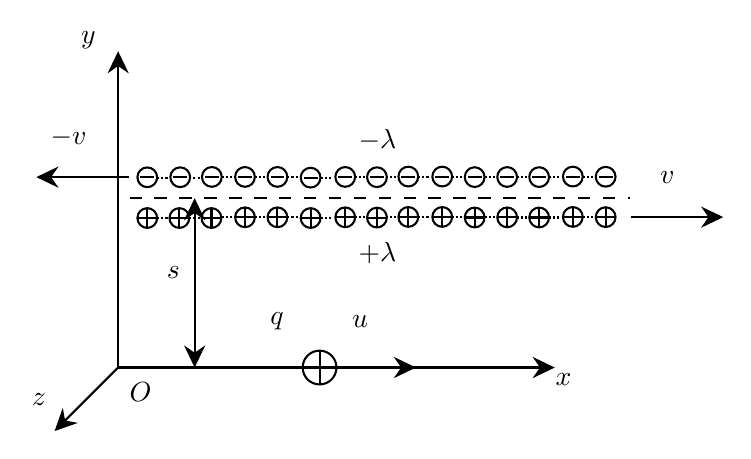
\begin{tikzpicture}[x=0.75pt,y=0.75pt,yscale=-1,xscale=1]
%uncomment if require: \path (0,300); %set diagram left start at 0, and has height of 300

%Flowchart: Or [id:dp6879817857375945] 
\draw   (420.67,165.27) .. controls (420.67,162.64) and (422.8,160.51) .. (425.43,160.51) .. controls (428.06,160.51) and (430.19,162.64) .. (430.19,165.27) .. controls (430.19,167.89) and (428.06,170.02) .. (425.43,170.02) .. controls (422.8,170.02) and (420.67,167.89) .. (420.67,165.27) -- cycle ; \draw   (420.67,165.27) -- (430.19,165.27) ; \draw   (425.43,160.51) -- (425.43,170.02) ;
%Flowchart: Or [id:dp03497399514177135] 
\draw   (404.86,165.18) .. controls (404.86,162.55) and (406.99,160.42) .. (409.61,160.42) .. controls (412.24,160.42) and (414.37,162.55) .. (414.37,165.18) .. controls (414.37,167.8) and (412.24,169.93) .. (409.61,169.93) .. controls (406.99,169.93) and (404.86,167.8) .. (404.86,165.18) -- cycle ; \draw   (404.86,165.18) -- (414.37,165.18) ; \draw   (409.61,160.42) -- (409.61,169.93) ;
%Flowchart: Or [id:dp026755679237013386] 
\draw   (388.63,165.44) .. controls (388.63,162.81) and (390.75,160.68) .. (393.38,160.68) .. controls (396.01,160.68) and (398.14,162.81) .. (398.14,165.44) .. controls (398.14,168.07) and (396.01,170.2) .. (393.38,170.2) .. controls (390.75,170.2) and (388.63,168.07) .. (388.63,165.44) -- cycle ; \draw   (388.63,165.44) -- (398.14,165.44) ; \draw   (393.38,160.68) -- (393.38,170.2) ;
%Flowchart: Or [id:dp6836213609351465] 
\draw   (373.22,165.38) .. controls (373.22,162.76) and (375.35,160.63) .. (377.98,160.63) .. controls (380.61,160.63) and (382.73,162.76) .. (382.73,165.38) .. controls (382.73,168.01) and (380.61,170.14) .. (377.98,170.14) .. controls (375.35,170.14) and (373.22,168.01) .. (373.22,165.38) -- cycle ; \draw   (373.22,165.38) -- (382.73,165.38) ; \draw   (377.98,160.63) -- (377.98,170.14) ;
%Flowchart: Or [id:dp010217150333981628] 
\draw   (357.56,165.44) .. controls (357.56,162.81) and (359.69,160.68) .. (362.32,160.68) .. controls (364.94,160.68) and (367.07,162.81) .. (367.07,165.44) .. controls (367.07,168.07) and (364.94,170.2) .. (362.32,170.2) .. controls (359.69,170.2) and (357.56,168.07) .. (357.56,165.44) -- cycle ; \draw   (357.56,165.44) -- (367.07,165.44) ; \draw   (362.32,160.68) -- (362.32,170.2) ;
%Flowchart: Or [id:dp408099385861058] 
\draw   (341.93,165.18) .. controls (341.93,162.55) and (344.06,160.42) .. (346.68,160.42) .. controls (349.31,160.42) and (351.44,162.55) .. (351.44,165.18) .. controls (351.44,167.81) and (349.31,169.93) .. (346.68,169.93) .. controls (344.06,169.93) and (341.93,167.81) .. (341.93,165.18) -- cycle ; \draw   (341.93,165.18) -- (351.44,165.18) ; \draw   (346.68,160.42) -- (346.68,169.93) ;
%Flowchart: Or [id:dp0501918076730552] 
\draw   (325.6,165.18) .. controls (325.6,162.55) and (327.73,160.42) .. (330.35,160.42) .. controls (332.98,160.42) and (335.11,162.55) .. (335.11,165.18) .. controls (335.11,167.81) and (332.98,169.93) .. (330.35,169.93) .. controls (327.73,169.93) and (325.6,167.81) .. (325.6,165.18) -- cycle ; \draw   (325.6,165.18) -- (335.11,165.18) ; \draw   (330.35,160.42) -- (330.35,169.93) ;
%Flowchart: Or [id:dp7362406071517613] 
\draw   (310.49,165.48) .. controls (310.49,162.86) and (312.61,160.73) .. (315.24,160.73) .. controls (317.87,160.73) and (320,162.86) .. (320,165.48) .. controls (320,168.11) and (317.87,170.24) .. (315.24,170.24) .. controls (312.61,170.24) and (310.49,168.11) .. (310.49,165.48) -- cycle ; \draw   (310.49,165.48) -- (320,165.48) ; \draw   (315.24,160.73) -- (315.24,170.24) ;
%Flowchart: Or [id:dp5402812040058182] 
\draw   (295.2,165.35) .. controls (295.2,162.73) and (297.33,160.6) .. (299.95,160.6) .. controls (302.58,160.6) and (304.71,162.73) .. (304.71,165.35) .. controls (304.71,167.98) and (302.58,170.11) .. (299.95,170.11) .. controls (297.33,170.11) and (295.2,167.98) .. (295.2,165.35) -- cycle ; \draw   (295.2,165.35) -- (304.71,165.35) ; \draw   (299.95,160.6) -- (299.95,170.11) ;
%Flowchart: Or [id:dp7543529230911408] 
\draw   (278.52,165.7) .. controls (278.52,163.07) and (280.65,160.94) .. (283.28,160.94) .. controls (285.9,160.94) and (288.03,163.07) .. (288.03,165.7) .. controls (288.03,168.33) and (285.9,170.46) .. (283.28,170.46) .. controls (280.65,170.46) and (278.52,168.33) .. (278.52,165.7) -- cycle ; \draw   (278.52,165.7) -- (288.03,165.7) ; \draw   (283.28,160.94) -- (283.28,170.46) ;
%Flowchart: Or [id:dp45508661857855137] 
\draw   (262.54,165.35) .. controls (262.54,162.73) and (264.67,160.6) .. (267.3,160.6) .. controls (269.92,160.6) and (272.05,162.73) .. (272.05,165.35) .. controls (272.05,167.98) and (269.92,170.11) .. (267.3,170.11) .. controls (264.67,170.11) and (262.54,167.98) .. (262.54,165.35) -- cycle ; \draw   (262.54,165.35) -- (272.05,165.35) ; \draw   (267.3,160.6) -- (267.3,170.11) ;
%Flowchart: Or [id:dp028955662135914828] 
\draw   (246.91,165.35) .. controls (246.91,162.73) and (249.04,160.6) .. (251.66,160.6) .. controls (254.29,160.6) and (256.42,162.73) .. (256.42,165.35) .. controls (256.42,167.98) and (254.29,170.11) .. (251.66,170.11) .. controls (249.04,170.11) and (246.91,167.98) .. (246.91,165.35) -- cycle ; \draw   (246.91,165.35) -- (256.42,165.35) ; \draw   (251.66,160.6) -- (251.66,170.11) ;
%Flowchart: Or [id:dp9877029132095312] 
\draw   (230.75,165.7) .. controls (230.75,163.07) and (232.88,160.94) .. (235.51,160.94) .. controls (238.13,160.94) and (240.26,163.07) .. (240.26,165.7) .. controls (240.26,168.33) and (238.13,170.46) .. (235.51,170.46) .. controls (232.88,170.46) and (230.75,168.33) .. (230.75,165.7) -- cycle ; \draw   (230.75,165.7) -- (240.26,165.7) ; \draw   (235.51,160.94) -- (235.51,170.46) ;
%Flowchart: Or [id:dp8939416554833004] 
\draw   (215.29,165.7) .. controls (215.29,163.07) and (217.42,160.94) .. (220.05,160.94) .. controls (222.67,160.94) and (224.8,163.07) .. (224.8,165.7) .. controls (224.8,168.33) and (222.67,170.46) .. (220.05,170.46) .. controls (217.42,170.46) and (215.29,168.33) .. (215.29,165.7) -- cycle ; \draw   (215.29,165.7) -- (224.8,165.7) ; \draw   (220.05,160.94) -- (220.05,170.46) ;
%Flowchart: Or [id:dp47940366097006293] 
\draw   (199.83,165.7) .. controls (199.83,163.07) and (201.96,160.94) .. (204.59,160.94) .. controls (207.21,160.94) and (209.34,163.07) .. (209.34,165.7) .. controls (209.34,168.33) and (207.21,170.46) .. (204.59,170.46) .. controls (201.96,170.46) and (199.83,168.33) .. (199.83,165.7) -- cycle ; \draw   (199.83,165.7) -- (209.34,165.7) ; \draw   (204.59,160.94) -- (204.59,170.46) ;
%Straight Lines [id:da9536544579342703] 
\draw    (190.55,237.73) -- (190.55,88.33) ;
\draw [shift={(190.55,85.33)}, rotate = 450] [fill={rgb, 255:red, 0; green, 0; blue, 0 }  ][line width=0.08]  [draw opacity=0] (10.72,-5.15) -- (0,0) -- (10.72,5.15) -- (7.12,0) -- cycle    ;
%Straight Lines [id:da43116579994994186] 
\draw    (190.55,237.73) -- (397.91,237.73) ;
\draw [shift={(400.91,237.73)}, rotate = 180] [fill={rgb, 255:red, 0; green, 0; blue, 0 }  ][line width=0.08]  [draw opacity=0] (10.72,-5.15) -- (0,0) -- (10.72,5.15) -- (7.12,0) -- cycle    ;
%Straight Lines [id:da7407186216980959] 
\draw    (190.55,237.73) -- (162.07,266.21) ;
\draw [shift={(159.95,268.33)}, rotate = 315] [fill={rgb, 255:red, 0; green, 0; blue, 0 }  ][line width=0.08]  [draw opacity=0] (10.72,-5.15) -- (0,0) -- (10.72,5.15) -- (7.12,0) -- cycle    ;
%Straight Lines [id:da5551157434877387] 
\draw    (227.41,159.13) -- (227.41,234.74) ;
\draw [shift={(227.41,237.74)}, rotate = 270] [fill={rgb, 255:red, 0; green, 0; blue, 0 }  ][line width=0.08]  [draw opacity=0] (10.72,-5.15) -- (0,0) -- (10.72,5.15) -- (7.12,0) -- cycle    ;
\draw [shift={(227.41,156.13)}, rotate = 90] [fill={rgb, 255:red, 0; green, 0; blue, 0 }  ][line width=0.08]  [draw opacity=0] (10.72,-5.15) -- (0,0) -- (10.72,5.15) -- (7.12,0) -- cycle    ;
%Straight Lines [id:da20959782887712985] 
\draw    (154.14,145.99) -- (195.72,145.99) ;
\draw [shift={(151.14,145.99)}, rotate = 0] [fill={rgb, 255:red, 0; green, 0; blue, 0 }  ][line width=0.08]  [draw opacity=0] (10.72,-5.15) -- (0,0) -- (10.72,5.15) -- (7.12,0) -- cycle    ;
%Flowchart: Connector [id:dp5192915337241915] 
\draw   (209.34,146.07) .. controls (209.34,143.44) and (207.21,141.32) .. (204.59,141.32) .. controls (201.96,141.32) and (199.83,143.44) .. (199.83,146.07) .. controls (199.83,148.7) and (201.96,150.83) .. (204.59,150.83) .. controls (207.21,150.83) and (209.34,148.7) .. (209.34,146.07) -- cycle ;
%Straight Lines [id:da09728624693545451] 
\draw    (207.92,146.07) -- (201.26,146.07) ;

%Flowchart: Connector [id:dp9269629464427493] 
\draw   (225.21,146.04) .. controls (225.21,143.42) and (223.08,141.29) .. (220.45,141.29) .. controls (217.83,141.29) and (215.7,143.42) .. (215.7,146.04) .. controls (215.7,148.67) and (217.83,150.8) .. (220.45,150.8) .. controls (223.08,150.8) and (225.21,148.67) .. (225.21,146.04) -- cycle ;
%Straight Lines [id:da9056860464426539] 
\draw    (223.78,146.04) -- (217.12,146.04) ;

%Flowchart: Connector [id:dp23794505798383025] 
\draw   (240.44,145.9) .. controls (240.44,143.27) and (238.31,141.14) .. (235.68,141.14) .. controls (233.06,141.14) and (230.93,143.27) .. (230.93,145.9) .. controls (230.93,148.52) and (233.06,150.65) .. (235.68,150.65) .. controls (238.31,150.65) and (240.44,148.52) .. (240.44,145.9) -- cycle ;
%Straight Lines [id:da5271358117711293] 
\draw    (239.01,145.9) -- (232.35,145.9) ;

%Flowchart: Connector [id:dp3448684120857046] 
\draw   (256.42,145.9) .. controls (256.42,143.27) and (254.29,141.14) .. (251.66,141.14) .. controls (249.04,141.14) and (246.91,143.27) .. (246.91,145.9) .. controls (246.91,148.52) and (249.04,150.65) .. (251.66,150.65) .. controls (254.29,150.65) and (256.42,148.52) .. (256.42,145.9) -- cycle ;
%Straight Lines [id:da8328674698396767] 
\draw    (254.99,145.9) -- (248.33,145.9) ;

%Flowchart: Connector [id:dp8761268211573081] 
\draw   (272.05,145.9) .. controls (272.05,143.27) and (269.92,141.14) .. (267.3,141.14) .. controls (264.67,141.14) and (262.54,143.27) .. (262.54,145.9) .. controls (262.54,148.52) and (264.67,150.65) .. (267.3,150.65) .. controls (269.92,150.65) and (272.05,148.52) .. (272.05,145.9) -- cycle ;
%Straight Lines [id:da30730771162610204] 
\draw    (270.63,145.9) -- (263.97,145.9) ;

%Flowchart: Connector [id:dp6774596821155621] 
\draw   (288.03,146.24) .. controls (288.03,143.62) and (285.9,141.49) .. (283.28,141.49) .. controls (280.65,141.49) and (278.52,143.62) .. (278.52,146.24) .. controls (278.52,148.87) and (280.65,151) .. (283.28,151) .. controls (285.9,151) and (288.03,148.87) .. (288.03,146.24) -- cycle ;
%Straight Lines [id:da09935306117639353] 
\draw    (286.61,146.24) -- (279.95,146.24) ;

%Flowchart: Connector [id:dp5822382729949567] 
\draw   (304.71,145.9) .. controls (304.71,143.27) and (302.58,141.14) .. (299.95,141.14) .. controls (297.33,141.14) and (295.2,143.27) .. (295.2,145.9) .. controls (295.2,148.52) and (297.33,150.65) .. (299.95,150.65) .. controls (302.58,150.65) and (304.71,148.52) .. (304.71,145.9) -- cycle ;
%Straight Lines [id:da22968727436940273] 
\draw    (303.28,145.9) -- (296.63,145.9) ;

%Flowchart: Connector [id:dp4368679506811972] 
\draw   (320,146.03) .. controls (320,143.4) and (317.87,141.27) .. (315.24,141.27) .. controls (312.61,141.27) and (310.49,143.4) .. (310.49,146.03) .. controls (310.49,148.66) and (312.61,150.78) .. (315.24,150.78) .. controls (317.87,150.78) and (320,148.66) .. (320,146.03) -- cycle ;
%Straight Lines [id:da21800720013539876] 
\draw    (318.57,146.03) -- (311.91,146.03) ;

%Flowchart: Connector [id:dp5444818407219238] 
\draw   (335.11,145.72) .. controls (335.11,143.1) and (332.98,140.97) .. (330.35,140.97) .. controls (327.73,140.97) and (325.6,143.1) .. (325.6,145.72) .. controls (325.6,148.35) and (327.73,150.48) .. (330.35,150.48) .. controls (332.98,150.48) and (335.11,148.35) .. (335.11,145.72) -- cycle ;
%Straight Lines [id:da3200992195204113] 
\draw    (333.68,145.72) -- (327.02,145.72) ;

%Flowchart: Connector [id:dp5591662634072039] 
\draw   (351.44,145.72) .. controls (351.44,143.1) and (349.31,140.97) .. (346.68,140.97) .. controls (344.06,140.97) and (341.93,143.1) .. (341.93,145.72) .. controls (341.93,148.35) and (344.06,150.48) .. (346.68,150.48) .. controls (349.31,150.48) and (351.44,148.35) .. (351.44,145.72) -- cycle ;
%Straight Lines [id:da0683806945402019] 
\draw    (350.01,145.72) -- (343.35,145.72) ;

%Flowchart: Connector [id:dp3770795025892877] 
\draw   (367.07,145.98) .. controls (367.07,143.36) and (364.94,141.23) .. (362.32,141.23) .. controls (359.69,141.23) and (357.56,143.36) .. (357.56,145.98) .. controls (357.56,148.61) and (359.69,150.74) .. (362.32,150.74) .. controls (364.94,150.74) and (367.07,148.61) .. (367.07,145.98) -- cycle ;
%Straight Lines [id:da12440075706322573] 
\draw    (365.65,145.98) -- (358.99,145.98) ;

%Flowchart: Connector [id:dp37451727498060494] 
\draw   (382.73,145.93) .. controls (382.73,143.3) and (380.61,141.17) .. (377.98,141.17) .. controls (375.35,141.17) and (373.22,143.3) .. (373.22,145.93) .. controls (373.22,148.55) and (375.35,150.68) .. (377.98,150.68) .. controls (380.61,150.68) and (382.73,148.55) .. (382.73,145.93) -- cycle ;
%Straight Lines [id:da088070937769539] 
\draw    (381.31,145.93) -- (374.65,145.93) ;

%Flowchart: Connector [id:dp2972231699800687] 
\draw   (398.14,145.98) .. controls (398.14,143.36) and (396.01,141.23) .. (393.38,141.23) .. controls (390.75,141.23) and (388.63,143.36) .. (388.63,145.98) .. controls (388.63,148.61) and (390.75,150.74) .. (393.38,150.74) .. controls (396.01,150.74) and (398.14,148.61) .. (398.14,145.98) -- cycle ;
%Straight Lines [id:da1788907731369631] 
\draw    (396.71,145.98) -- (390.05,145.98) ;

%Flowchart: Connector [id:dp46132865419269] 
\draw   (414.37,145.72) .. controls (414.37,143.09) and (412.24,140.97) .. (409.61,140.97) .. controls (406.99,140.97) and (404.86,143.09) .. (404.86,145.72) .. controls (404.86,148.35) and (406.99,150.48) .. (409.61,150.48) .. controls (412.24,150.48) and (414.37,148.35) .. (414.37,145.72) -- cycle ;
%Straight Lines [id:da1601026319187211] 
\draw    (412.94,145.72) -- (406.28,145.72) ;

%Flowchart: Connector [id:dp4186087152378848] 
\draw   (430.19,145.81) .. controls (430.19,143.18) and (428.06,141.05) .. (425.43,141.05) .. controls (422.8,141.05) and (420.67,143.18) .. (420.67,145.81) .. controls (420.67,148.44) and (422.8,150.57) .. (425.43,150.57) .. controls (428.06,150.57) and (430.19,148.44) .. (430.19,145.81) -- cycle ;
%Straight Lines [id:da7148840376699521] 
\draw    (428.76,145.81) -- (422.1,145.81) ;

%Straight Lines [id:da6449560491326731] 
\draw  [dash pattern={on 0.75pt off 0.75pt on 0.75pt off 0.75pt}]  (209.34,146.24) -- (215.29,146.24) ;
%Straight Lines [id:da00721159434487606] 
\draw  [dash pattern={on 0.75pt off 0.75pt on 0.75pt off 0.75pt}]  (224.8,146.24) -- (230.75,146.24) ;
%Straight Lines [id:da13178385048545538] 
\draw  [dash pattern={on 0.75pt off 0.75pt on 0.75pt off 0.75pt}]  (240.44,145.9) -- (246.39,145.9) ;
%Straight Lines [id:da7513017506304862] 
\draw  [dash pattern={on 0.75pt off 0.75pt on 0.75pt off 0.75pt}]  (256.42,145.9) -- (262.37,145.9) ;
%Straight Lines [id:da7439687697280251] 
\draw  [dash pattern={on 0.75pt off 0.75pt on 0.75pt off 0.75pt}]  (272.05,145.9) -- (278,145.9) ;
%Straight Lines [id:da552990550031649] 
\draw  [dash pattern={on 0.75pt off 0.75pt on 0.75pt off 0.75pt}]  (288.03,146.24) -- (293.98,146.24) ;
%Straight Lines [id:da7882847758763452] 
\draw  [dash pattern={on 0.75pt off 0.75pt on 0.75pt off 0.75pt}]  (304.71,145.9) -- (310.66,145.9) ;
%Straight Lines [id:da65426455583666] 
\draw  [dash pattern={on 0.75pt off 0.75pt on 0.75pt off 0.75pt}]  (319.65,145.72) -- (325.6,145.72) ;
%Straight Lines [id:da9919793099444005] 
\draw  [dash pattern={on 0.75pt off 0.75pt on 0.75pt off 0.75pt}]  (335.11,145.72) -- (341.06,145.72) ;
%Straight Lines [id:da9882620156007165] 
\draw  [dash pattern={on 0.75pt off 0.75pt on 0.75pt off 0.75pt}]  (351.44,145.72) -- (357.39,145.72) ;
%Straight Lines [id:da5078108911166326] 
\draw  [dash pattern={on 0.75pt off 0.75pt on 0.75pt off 0.75pt}]  (367.27,145.93) -- (373.22,145.93) ;
%Straight Lines [id:da3820500507998674] 
\draw  [dash pattern={on 0.75pt off 0.75pt on 0.75pt off 0.75pt}]  (382.68,145.98) -- (388.63,145.98) ;
%Straight Lines [id:da3916015047841639] 
\draw  [dash pattern={on 0.75pt off 0.75pt on 0.75pt off 0.75pt}]  (398.14,145.98) -- (404.09,145.98) ;
%Straight Lines [id:da382537053948959] 
\draw  [dash pattern={on 0.75pt off 0.75pt on 0.75pt off 0.75pt}]  (414.37,145.72) -- (420.32,145.72) ;
%Straight Lines [id:da05742407375026293] 
\draw  [dash pattern={on 0.75pt off 0.75pt on 0.75pt off 0.75pt}]  (209.34,165.7) -- (215.29,165.7) ;
%Straight Lines [id:da04611174975326349] 
\draw  [dash pattern={on 0.75pt off 0.75pt on 0.75pt off 0.75pt}]  (224.8,165.7) -- (230.75,165.7) ;
%Straight Lines [id:da6190332896191486] 
\draw  [dash pattern={on 0.75pt off 0.75pt on 0.75pt off 0.75pt}]  (240.44,165.35) -- (246.39,165.35) ;
%Straight Lines [id:da3227411243905076] 
\draw  [dash pattern={on 0.75pt off 0.75pt on 0.75pt off 0.75pt}]  (256.42,165.35) -- (262.37,165.35) ;
%Straight Lines [id:da20284390404807429] 
\draw  [dash pattern={on 0.75pt off 0.75pt on 0.75pt off 0.75pt}]  (272.05,165.35) -- (278,165.35) ;
%Straight Lines [id:da33214261590506067] 
\draw  [dash pattern={on 0.75pt off 0.75pt on 0.75pt off 0.75pt}]  (288.03,165.7) -- (293.98,165.7) ;
%Straight Lines [id:da766103105135199] 
\draw  [dash pattern={on 0.75pt off 0.75pt on 0.75pt off 0.75pt}]  (304.71,165.35) -- (310.66,165.35) ;
%Straight Lines [id:da5301265822166792] 
\draw  [dash pattern={on 0.75pt off 0.75pt on 0.75pt off 0.75pt}]  (319.65,165.18) -- (325.6,165.18) ;
%Straight Lines [id:da697818272305337] 
\draw  [dash pattern={on 0.75pt off 0.75pt on 0.75pt off 0.75pt}]  (335.11,165.18) -- (341.06,165.18) ;
%Straight Lines [id:da7742922246294379] 
\draw  [dash pattern={on 0.75pt off 0.75pt on 0.75pt off 0.75pt}]  (351.44,165.18) -- (357.39,165.18) ;
%Straight Lines [id:da9621236933484416] 
\draw  [dash pattern={on 0.75pt off 0.75pt on 0.75pt off 0.75pt}]  (367.27,165.38) -- (373.22,165.38) ;
%Straight Lines [id:da9920094970183546] 
\draw  [dash pattern={on 0.75pt off 0.75pt on 0.75pt off 0.75pt}]  (382.68,165.44) -- (388.63,165.44) ;
%Straight Lines [id:da2854228330117363] 
\draw  [dash pattern={on 0.75pt off 0.75pt on 0.75pt off 0.75pt}]  (398.14,165.44) -- (404.09,165.44) ;
%Straight Lines [id:da08453948854200788] 
\draw  [dash pattern={on 0.75pt off 0.75pt on 0.75pt off 0.75pt}]  (414.37,165.18) -- (420.32,165.18) ;
%Straight Lines [id:da3852099469662127] 
\draw  [dash pattern={on 4.5pt off 4.5pt}]  (196.05,156.04) -- (437.39,156.04) ;
%Straight Lines [id:da4817537127190876] 
\draw    (437.48,165.27) -- (479.07,165.27) ;
\draw [shift={(482.07,165.27)}, rotate = 180] [fill={rgb, 255:red, 0; green, 0; blue, 0 }  ][line width=0.08]  [draw opacity=0] (10.72,-5.15) -- (0,0) -- (10.72,5.15) -- (7.12,0) -- cycle    ;
%Flowchart: Or [id:dp3032664453712228] 
\draw   (279.45,237.73) .. controls (279.45,233.24) and (283.1,229.59) .. (287.59,229.59) .. controls (292.09,229.59) and (295.73,233.24) .. (295.73,237.73) .. controls (295.73,242.23) and (292.09,245.87) .. (287.59,245.87) .. controls (283.1,245.87) and (279.45,242.23) .. (279.45,237.73) -- cycle ; \draw   (279.45,237.73) -- (295.73,237.73) ; \draw   (287.59,229.59) -- (287.59,245.87) ;
%Straight Lines [id:da47642651899131216] 
\draw    (295.73,237.73) -- (331.03,237.73) ;
\draw [shift={(334.03,237.73)}, rotate = 180] [fill={rgb, 255:red, 0; green, 0; blue, 0 }  ][line width=0.08]  [draw opacity=0] (10.72,-5.15) -- (0,0) -- (10.72,5.15) -- (7.12,0) -- cycle    ;

% Text Node
\draw (212.52,187.78) node [anchor=north west][inner sep=0.75pt]    {$s$};
% Text Node
\draw (399.77,239.25) node [anchor=north west][inner sep=0.75pt]    {$x$};
% Text Node
\draw (171.17,74.49) node [anchor=north west][inner sep=0.75pt]    {$y$};
% Text Node
\draw (147.46,248.98) node [anchor=north west][inner sep=0.75pt]    {$z$};
% Text Node
\draw (194.6,243.51) node [anchor=north west][inner sep=0.75pt]    {$O$};
% Text Node
\draw (450.17,141.85) node [anchor=north west][inner sep=0.75pt]    {$\ot{v}$};
% Text Node
\draw (156.47,120.91) node [anchor=north west][inner sep=0.75pt]    {$-\ot{v}$};
% Text Node
\draw (304.87,175.88) node [anchor=north west][inner sep=0.75pt]    {$+\lambda$};
% Text Node
\draw (304.87,121.65) node [anchor=north west][inner sep=0.75pt]    {$-\lambda$};
% Text Node
\draw (301.82,211.16) node [anchor=north west][inner sep=0.75pt]    {$\ot{u}$};
% Text Node
\draw (262.37,209.66) node [anchor=north west][inner sep=0.75pt]    {$q$};
\end{tikzpicture}
\\Hình a.
\end{center}
\begin{enumerate}[1.]
    \item Xác định độ lớn lực từ, lực điện tác dụng lên điện tích $q$ trong hệ quy chiếu ${K}$.
    \item Xét bài toán trong hệ quy chiếu ${K}^{\prime}$ gắn với điện tích $q$. Gọi vận tốc của điện tích âm và điện tích dương trên hai dây khi đó tương ứng là $\overrightarrow{{v}_{n}}$ và $\overrightarrow{{v}_{p}}$ (Hình $b$). Do hiệu ứng tương đối tính, hai dây đã cho tương đương với một dây không trung hòa với mật độ điện tích dài tổng cộng $\lambda_{\mathrm{T}}=\lambda_{\mathrm{p}}+\lambda_{\mathrm{n}}$. Trong $\lambda_{\mathrm{p}}$ và $\lambda_{\mathrm{n}}$ tương ứng là mật độ điện tích dài của dây tích điện dương và dây tích điện âm trong hệ quy chiếu ${K}^{\prime}$. Biết rằng, điện tích bất biến với phép biến đổi Lorentz.
    \begin{center}
    
\tikzset{every picture/.style={line width=0.75pt}} %set default line width to 0.75pt        

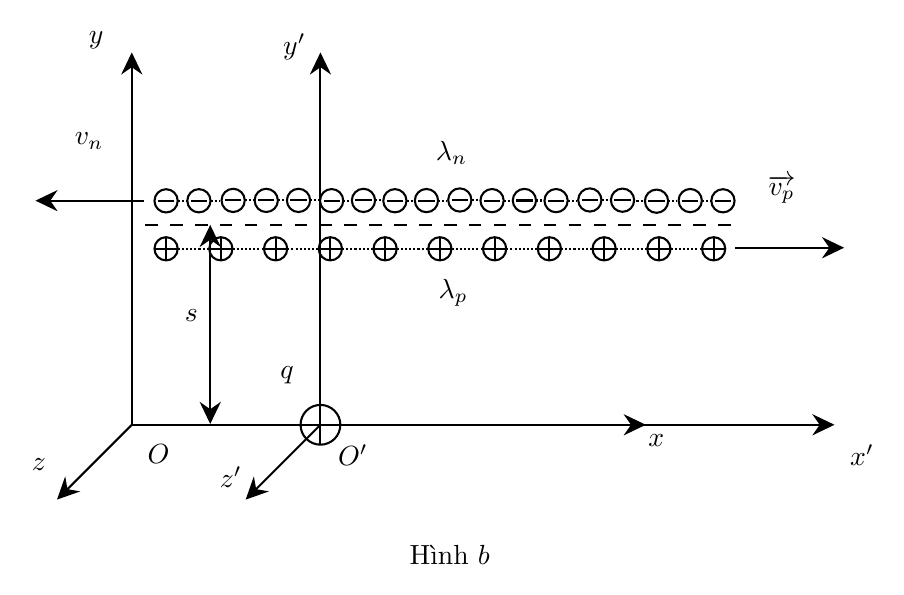
\begin{tikzpicture}[x=0.75pt,y=0.75pt,yscale=-1,xscale=1]
%uncomment if require: \path (0,714); %set diagram left start at 0, and has height of 714

%Flowchart: Or [id:dp48495376245484234] 
\draw   (419.42,145.41) .. controls (419.42,142.32) and (421.92,139.82) .. (425.02,139.82) .. controls (428.11,139.82) and (430.61,142.32) .. (430.61,145.41) .. controls (430.61,148.51) and (428.11,151.01) .. (425.02,151.01) .. controls (421.92,151.01) and (419.42,148.51) .. (419.42,145.41) -- cycle ; \draw   (419.42,145.41) -- (430.61,145.41) ; \draw   (425.02,139.82) -- (425.02,151.01) ;
%Flowchart: Or [id:dp07246846880156754] 
\draw   (393.04,145.41) .. controls (393.04,142.32) and (395.54,139.82) .. (398.64,139.82) .. controls (401.73,139.82) and (404.23,142.32) .. (404.23,145.41) .. controls (404.23,148.51) and (401.73,151.01) .. (398.64,151.01) .. controls (395.54,151.01) and (393.04,148.51) .. (393.04,145.41) -- cycle ; \draw   (393.04,145.41) -- (404.23,145.41) ; \draw   (398.64,139.82) -- (398.64,151.01) ;
%Flowchart: Or [id:dp3361276651937999] 
\draw   (366.66,145.41) .. controls (366.66,142.32) and (369.16,139.82) .. (372.25,139.82) .. controls (375.35,139.82) and (377.85,142.32) .. (377.85,145.41) .. controls (377.85,148.51) and (375.35,151.01) .. (372.25,151.01) .. controls (369.16,151.01) and (366.66,148.51) .. (366.66,145.41) -- cycle ; \draw   (366.66,145.41) -- (377.85,145.41) ; \draw   (372.25,139.82) -- (372.25,151.01) ;
%Flowchart: Or [id:dp3048217345673483] 
\draw   (340.28,145.41) .. controls (340.28,142.32) and (342.78,139.82) .. (345.87,139.82) .. controls (348.97,139.82) and (351.47,142.32) .. (351.47,145.41) .. controls (351.47,148.51) and (348.97,151.01) .. (345.87,151.01) .. controls (342.78,151.01) and (340.28,148.51) .. (340.28,145.41) -- cycle ; \draw   (340.28,145.41) -- (351.47,145.41) ; \draw   (345.87,139.82) -- (345.87,151.01) ;
%Flowchart: Or [id:dp8492740101331999] 
\draw   (313.89,145.41) .. controls (313.89,142.32) and (316.4,139.82) .. (319.49,139.82) .. controls (322.59,139.82) and (325.09,142.32) .. (325.09,145.41) .. controls (325.09,148.51) and (322.59,151.01) .. (319.49,151.01) .. controls (316.4,151.01) and (313.89,148.51) .. (313.89,145.41) -- cycle ; \draw   (313.89,145.41) -- (325.09,145.41) ; \draw   (319.49,139.82) -- (319.49,151.01) ;
%Flowchart: Or [id:dp6766304049326974] 
\draw   (287.51,145.41) .. controls (287.51,142.32) and (290.02,139.82) .. (293.11,139.82) .. controls (296.2,139.82) and (298.71,142.32) .. (298.71,145.41) .. controls (298.71,148.51) and (296.2,151.01) .. (293.11,151.01) .. controls (290.02,151.01) and (287.51,148.51) .. (287.51,145.41) -- cycle ; \draw   (287.51,145.41) -- (298.71,145.41) ; \draw   (293.11,139.82) -- (293.11,151.01) ;
%Flowchart: Or [id:dp36613883539189107] 
\draw   (261.13,145.41) .. controls (261.13,142.32) and (263.64,139.82) .. (266.73,139.82) .. controls (269.82,139.82) and (272.33,142.32) .. (272.33,145.41) .. controls (272.33,148.51) and (269.82,151.01) .. (266.73,151.01) .. controls (263.64,151.01) and (261.13,148.51) .. (261.13,145.41) -- cycle ; \draw   (261.13,145.41) -- (272.33,145.41) ; \draw   (266.73,139.82) -- (266.73,151.01) ;
%Flowchart: Or [id:dp5159162826013144] 
\draw   (234.75,145.41) .. controls (234.75,142.32) and (237.26,139.82) .. (240.35,139.82) .. controls (243.44,139.82) and (245.95,142.32) .. (245.95,145.41) .. controls (245.95,148.51) and (243.44,151.01) .. (240.35,151.01) .. controls (237.26,151.01) and (234.75,148.51) .. (234.75,145.41) -- cycle ; \draw   (234.75,145.41) -- (245.95,145.41) ; \draw   (240.35,139.82) -- (240.35,151.01) ;
%Flowchart: Or [id:dp9468858446036854] 
\draw   (208.37,145.41) .. controls (208.37,142.32) and (210.88,139.82) .. (213.97,139.82) .. controls (217.06,139.82) and (219.57,142.32) .. (219.57,145.41) .. controls (219.57,148.51) and (217.06,151.01) .. (213.97,151.01) .. controls (210.88,151.01) and (208.37,148.51) .. (208.37,145.41) -- cycle ; \draw   (208.37,145.41) -- (219.57,145.41) ; \draw   (213.97,139.82) -- (213.97,151.01) ;
%Flowchart: Or [id:dp1584941590683897] 
\draw   (181.99,145.41) .. controls (181.99,142.32) and (184.5,139.82) .. (187.59,139.82) .. controls (190.68,139.82) and (193.19,142.32) .. (193.19,145.41) .. controls (193.19,148.51) and (190.68,151.01) .. (187.59,151.01) .. controls (184.5,151.01) and (181.99,148.51) .. (181.99,145.41) -- cycle ; \draw   (181.99,145.41) -- (193.19,145.41) ; \draw   (187.59,139.82) -- (187.59,151.01) ;
%Flowchart: Or [id:dp9781477603019642] 
\draw   (155.61,145.41) .. controls (155.61,142.32) and (158.12,139.82) .. (161.21,139.82) .. controls (164.3,139.82) and (166.81,142.32) .. (166.81,145.41) .. controls (166.81,148.51) and (164.3,151.01) .. (161.21,151.01) .. controls (158.12,151.01) and (155.61,148.51) .. (155.61,145.41) -- cycle ; \draw   (155.61,145.41) -- (166.81,145.41) ; \draw   (161.21,139.82) -- (161.21,151.01) ;
%Straight Lines [id:da13407766104221497] 
\draw    (144.68,230.21) -- (144.68,53.8) ;
\draw [shift={(144.68,50.8)}, rotate = 450] [fill={rgb, 255:red, 0; green, 0; blue, 0 }  ][line width=0.08]  [draw opacity=0] (10.72,-5.15) -- (0,0) -- (10.72,5.15) -- (7.12,0) -- cycle    ;
%Straight Lines [id:da09372911592754574] 
\draw    (144.68,230.21) -- (389.33,230.21) ;
\draw [shift={(392.33,230.21)}, rotate = 180] [fill={rgb, 255:red, 0; green, 0; blue, 0 }  ][line width=0.08]  [draw opacity=0] (10.72,-5.15) -- (0,0) -- (10.72,5.15) -- (7.12,0) -- cycle    ;
%Straight Lines [id:da879705170446023] 
\draw    (144.68,230.21) -- (110.78,264.12) ;
\draw [shift={(108.66,266.24)}, rotate = 315] [fill={rgb, 255:red, 0; green, 0; blue, 0 }  ][line width=0.08]  [draw opacity=0] (10.72,-5.15) -- (0,0) -- (10.72,5.15) -- (7.12,0) -- cycle    ;
%Straight Lines [id:da0946098486653617] 
\draw    (182.48,136.91) -- (182.48,226.82) ;
\draw [shift={(182.48,229.82)}, rotate = 270] [fill={rgb, 255:red, 0; green, 0; blue, 0 }  ][line width=0.08]  [draw opacity=0] (10.72,-5.15) -- (0,0) -- (10.72,5.15) -- (7.12,0) -- cycle    ;
\draw [shift={(182.48,133.91)}, rotate = 90] [fill={rgb, 255:red, 0; green, 0; blue, 0 }  ][line width=0.08]  [draw opacity=0] (10.72,-5.15) -- (0,0) -- (10.72,5.15) -- (7.12,0) -- cycle    ;
%Straight Lines [id:da3554778853666085] 
\draw    (101.28,122.22) -- (150.77,122.22) ;
\draw [shift={(98.28,122.22)}, rotate = 0] [fill={rgb, 255:red, 0; green, 0; blue, 0 }  ][line width=0.08]  [draw opacity=0] (10.72,-5.15) -- (0,0) -- (10.72,5.15) -- (7.12,0) -- cycle    ;
%Flowchart: Connector [id:dp449331475472293] 
\draw   (166.81,122.31) .. controls (166.81,119.21) and (164.3,116.71) .. (161.21,116.71) .. controls (158.12,116.71) and (155.61,119.21) .. (155.61,122.31) .. controls (155.61,125.4) and (158.12,127.91) .. (161.21,127.91) .. controls (164.3,127.91) and (166.81,125.4) .. (166.81,122.31) -- cycle ;
%Straight Lines [id:da8221831421284478] 
\draw    (165.13,122.31) -- (157.29,122.31) ;

%Flowchart: Connector [id:dp9052258002738052] 
\draw   (182.62,122.27) .. controls (182.62,119.18) and (180.12,116.67) .. (177.02,116.67) .. controls (173.93,116.67) and (171.43,119.18) .. (171.43,122.27) .. controls (171.43,125.36) and (173.93,127.87) .. (177.02,127.87) .. controls (180.12,127.87) and (182.62,125.36) .. (182.62,122.27) -- cycle ;
%Straight Lines [id:da06285949131595103] 
\draw    (180.94,122.27) -- (173.11,122.27) ;

%Flowchart: Connector [id:dp643810497712491] 
\draw   (199.12,122.1) .. controls (199.12,119.01) and (196.61,116.5) .. (193.52,116.5) .. controls (190.43,116.5) and (187.92,119.01) .. (187.92,122.1) .. controls (187.92,125.19) and (190.43,127.7) .. (193.52,127.7) .. controls (196.61,127.7) and (199.12,125.19) .. (199.12,122.1) -- cycle ;
%Straight Lines [id:da6972242921275309] 
\draw    (197.44,122.1) -- (189.6,122.1) ;

%Flowchart: Connector [id:dp2651000364010949] 
\draw   (215.07,122.1) .. controls (215.07,119.01) and (212.56,116.5) .. (209.47,116.5) .. controls (206.38,116.5) and (203.87,119.01) .. (203.87,122.1) .. controls (203.87,125.19) and (206.38,127.7) .. (209.47,127.7) .. controls (212.56,127.7) and (215.07,125.19) .. (215.07,122.1) -- cycle ;
%Straight Lines [id:da9154114804190838] 
\draw    (213.39,122.1) -- (205.55,122.1) ;

%Flowchart: Connector [id:dp7256202090522232] 
\draw   (230.61,122.1) .. controls (230.61,119.01) and (228.11,116.5) .. (225.01,116.5) .. controls (221.92,116.5) and (219.42,119.01) .. (219.42,122.1) .. controls (219.42,125.19) and (221.92,127.7) .. (225.01,127.7) .. controls (228.11,127.7) and (230.61,125.19) .. (230.61,122.1) -- cycle ;
%Straight Lines [id:da3838814448233294] 
\draw    (228.93,122.1) -- (221.09,122.1) ;

%Flowchart: Connector [id:dp7258442617751413] 
\draw   (246.56,122.22) .. controls (246.56,119.13) and (244.06,116.63) .. (240.97,116.63) .. controls (237.87,116.63) and (235.37,119.13) .. (235.37,122.22) .. controls (235.37,125.32) and (237.87,127.82) .. (240.97,127.82) .. controls (244.06,127.82) and (246.56,125.32) .. (246.56,122.22) -- cycle ;
%Straight Lines [id:da9582541492971206] 
\draw    (244.88,122.22) -- (237.05,122.22) ;

%Flowchart: Connector [id:dp46080257322522944] 
\draw   (261.9,122.1) .. controls (261.9,119.01) and (259.39,116.5) .. (256.3,116.5) .. controls (253.21,116.5) and (250.7,119.01) .. (250.7,122.1) .. controls (250.7,125.19) and (253.21,127.7) .. (256.3,127.7) .. controls (259.39,127.7) and (261.9,125.19) .. (261.9,122.1) -- cycle ;
%Straight Lines [id:da727932025672505] 
\draw    (260.22,122.1) -- (252.38,122.1) ;

%Flowchart: Connector [id:dp017945886366892427] 
\draw   (277.03,122.26) .. controls (277.03,119.16) and (274.53,116.66) .. (271.44,116.66) .. controls (268.34,116.66) and (265.84,119.16) .. (265.84,122.26) .. controls (265.84,125.35) and (268.34,127.86) .. (271.44,127.86) .. controls (274.53,127.86) and (277.03,125.35) .. (277.03,122.26) -- cycle ;
%Straight Lines [id:da6631561601981784] 
\draw    (275.35,122.26) -- (267.52,122.26) ;

%Flowchart: Connector [id:dp2495382355330782] 
\draw   (292.25,122.18) .. controls (292.25,119.09) and (289.74,116.58) .. (286.65,116.58) .. controls (283.56,116.58) and (281.05,119.09) .. (281.05,122.18) .. controls (281.05,125.28) and (283.56,127.78) .. (286.65,127.78) .. controls (289.74,127.78) and (292.25,125.28) .. (292.25,122.18) -- cycle ;
%Straight Lines [id:da35798961027886156] 
\draw    (290.57,122.18) -- (282.73,122.18) ;

%Flowchart: Connector [id:dp6604541699225273] 
\draw   (308.32,121.9) .. controls (308.32,118.81) and (305.82,116.3) .. (302.72,116.3) .. controls (299.63,116.3) and (297.13,118.81) .. (297.13,121.9) .. controls (297.13,124.99) and (299.63,127.5) .. (302.72,127.5) .. controls (305.82,127.5) and (308.32,124.99) .. (308.32,121.9) -- cycle ;
%Straight Lines [id:da33941235367011013] 
\draw    (306.64,121.9) -- (298.81,121.9) ;

%Flowchart: Connector [id:dp8748924461060292] 
\draw   (323.87,122.2) .. controls (323.87,119.11) and (321.36,116.61) .. (318.27,116.61) .. controls (315.17,116.61) and (312.67,119.11) .. (312.67,122.2) .. controls (312.67,125.3) and (315.17,127.8) .. (318.27,127.8) .. controls (321.36,127.8) and (323.87,125.3) .. (323.87,122.2) -- cycle ;
%Straight Lines [id:da7094849527462301] 
\draw    (322.19,122.2) -- (314.35,122.2) ;

%Flowchart: Connector [id:dp3316820469849455] 
\draw   (339.44,122.14) .. controls (339.44,119.04) and (336.93,116.54) .. (333.84,116.54) .. controls (330.75,116.54) and (328.24,119.04) .. (328.24,122.14) .. controls (328.24,125.23) and (330.75,127.73) .. (333.84,127.73) .. controls (336.93,127.73) and (339.44,125.23) .. (339.44,122.14) -- cycle ;
%Straight Lines [id:da32866612717037436] 
\draw    (337.76,122.14) -- (329.92,122.14) ;

%Flowchart: Connector [id:dp5206872507556708] 
\draw   (354.71,122.2) .. controls (354.71,119.11) and (352.2,116.61) .. (349.11,116.61) .. controls (346.02,116.61) and (343.51,119.11) .. (343.51,122.2) .. controls (343.51,125.3) and (346.02,127.8) .. (349.11,127.8) .. controls (352.2,127.8) and (354.71,125.3) .. (354.71,122.2) -- cycle ;
%Straight Lines [id:da5881710043341299] 
\draw    (353.03,122.2) -- (345.19,122.2) ;

%Flowchart: Connector [id:dp3816531763150395] 
\draw   (370.96,121.89) .. controls (370.96,118.8) and (368.45,116.3) .. (365.36,116.3) .. controls (362.27,116.3) and (359.76,118.8) .. (359.76,121.89) .. controls (359.76,124.99) and (362.27,127.49) .. (365.36,127.49) .. controls (368.45,127.49) and (370.96,124.99) .. (370.96,121.89) -- cycle ;
%Straight Lines [id:da9854642594915772] 
\draw    (369.28,121.89) -- (361.44,121.89) ;

%Flowchart: Connector [id:dp8391568606652038] 
\draw   (386.72,122) .. controls (386.72,118.91) and (384.21,116.4) .. (381.12,116.4) .. controls (378.02,116.4) and (375.52,118.91) .. (375.52,122) .. controls (375.52,125.09) and (378.02,127.6) .. (381.12,127.6) .. controls (384.21,127.6) and (386.72,125.09) .. (386.72,122) -- cycle ;
%Straight Lines [id:da8856760163879229] 
\draw    (385.04,122) -- (377.2,122) ;

%Straight Lines [id:da6235570515421456] 
\draw  [dash pattern={on 0.75pt off 0.75pt on 0.75pt off 0.75pt}]  (166.81,122.51) -- (170.88,122.51) ;
%Straight Lines [id:da39854170154316715] 
\draw  [dash pattern={on 0.75pt off 0.75pt on 0.75pt off 0.75pt}]  (166.81,145.41) -- (176.53,145.41) -- (181.99,145.41) ;
%Straight Lines [id:da6655042562519713] 
\draw  [dash pattern={on 0.75pt off 0.75pt on 0.75pt off 0.75pt}]  (185.01,145.41) -- (192.01,145.41) ;
%Straight Lines [id:da14004062838192] 
\draw  [dash pattern={on 4.5pt off 4.5pt}]  (151.16,134.04) -- (435.28,134.04) ;
%Straight Lines [id:da218041866243061] 
\draw    (435.39,144.9) -- (484.88,144.9) ;
\draw [shift={(487.88,144.9)}, rotate = 180] [fill={rgb, 255:red, 0; green, 0; blue, 0 }  ][line width=0.08]  [draw opacity=0] (10.72,-5.15) -- (0,0) -- (10.72,5.15) -- (7.12,0) -- cycle    ;
%Straight Lines [id:da7380652022438452] 
\draw  [dash pattern={on 0.75pt off 0.75pt on 0.75pt off 0.75pt}]  (193.19,145.41) -- (208.37,145.41) ;
%Straight Lines [id:da8800277013387703] 
\draw  [dash pattern={on 0.75pt off 0.75pt on 0.75pt off 0.75pt}]  (219.57,145.41) -- (234.75,145.41) ;
%Straight Lines [id:da47251047441197014] 
\draw  [dash pattern={on 0.75pt off 0.75pt on 0.75pt off 0.75pt}]  (245.95,145.41) -- (261.13,145.41) ;
%Straight Lines [id:da3677572941416529] 
\draw  [dash pattern={on 0.75pt off 0.75pt on 0.75pt off 0.75pt}]  (272.33,145.41) -- (287.51,145.41) ;
%Straight Lines [id:da035672210133092186] 
\draw  [dash pattern={on 0.75pt off 0.75pt on 0.75pt off 0.75pt}]  (298.71,145.41) -- (313.89,145.41) ;
%Straight Lines [id:da973490915352379] 
\draw  [dash pattern={on 0.75pt off 0.75pt on 0.75pt off 0.75pt}]  (325.09,145.41) -- (340.28,145.41) ;
%Straight Lines [id:da3855586734805603] 
\draw  [dash pattern={on 0.75pt off 0.75pt on 0.75pt off 0.75pt}]  (351.47,145.41) -- (366.66,145.41) ;
%Straight Lines [id:da2181957570695301] 
\draw  [dash pattern={on 0.75pt off 0.75pt on 0.75pt off 0.75pt}]  (377.85,145.41) -- (393.04,145.41) ;
%Straight Lines [id:da06649700013358228] 
\draw  [dash pattern={on 0.75pt off 0.75pt on 0.75pt off 0.75pt}]  (404.23,145.41) -- (419.42,145.41) ;
%Straight Lines [id:da40750471434960023] 
\draw  [dash pattern={on 0.75pt off 0.75pt on 0.75pt off 0.75pt}]  (182.62,122.27) -- (186.69,122.27) ;
%Straight Lines [id:da19644359271811274] 
\draw  [dash pattern={on 0.75pt off 0.75pt on 0.75pt off 0.75pt}]  (199.12,122.1) -- (203.19,122.1) ;
%Straight Lines [id:da6635754052406704] 
\draw  [dash pattern={on 0.75pt off 0.75pt on 0.75pt off 0.75pt}]  (215.07,122.1) -- (219.14,122.1) ;
%Straight Lines [id:da3598813747727334] 
\draw  [dash pattern={on 0.75pt off 0.75pt on 0.75pt off 0.75pt}]  (230.61,122.1) -- (234.68,122.1) ;
%Straight Lines [id:da366381723452774] 
\draw  [dash pattern={on 0.75pt off 0.75pt on 0.75pt off 0.75pt}]  (246.56,122.22) -- (250.63,122.22) ;
%Straight Lines [id:da7608462288859508] 
\draw  [dash pattern={on 0.75pt off 0.75pt on 0.75pt off 0.75pt}]  (261.9,122.1) -- (265.97,122.1) ;
%Straight Lines [id:da031930278581471905] 
\draw  [dash pattern={on 0.75pt off 0.75pt on 0.75pt off 0.75pt}]  (277.03,122.26) -- (281.1,122.26) ;
%Straight Lines [id:da426478464053734] 
\draw  [dash pattern={on 0.75pt off 0.75pt on 0.75pt off 0.75pt}]  (292.25,122.18) -- (296.32,122.18) ;
%Straight Lines [id:da13337639307043814] 
\draw  [dash pattern={on 0.75pt off 0.75pt on 0.75pt off 0.75pt}]  (308.32,121.9) -- (312.39,121.9) ;
%Straight Lines [id:da9254244137009595] 
\draw  [dash pattern={on 0.75pt off 0.75pt on 0.75pt off 0.75pt}]  (323.87,122.2) -- (327.93,122.2) ;
%Straight Lines [id:da4745582005428728] 
\draw  [dash pattern={on 0.75pt off 0.75pt on 0.75pt off 0.75pt}]  (339.44,122.14) -- (343.51,122.14) ;
%Straight Lines [id:da36490330518835923] 
\draw  [dash pattern={on 0.75pt off 0.75pt on 0.75pt off 0.75pt}]  (354.71,122.2) -- (358.78,122.2) ;
%Straight Lines [id:da5643825179097741] 
\draw  [dash pattern={on 0.75pt off 0.75pt on 0.75pt off 0.75pt}]  (370.96,121.89) -- (375.03,121.89) ;
%Flowchart: Connector [id:dp919978816732206] 
\draw   (403.1,122.49) .. controls (403.1,119.4) and (400.59,116.89) .. (397.5,116.89) .. controls (394.4,116.89) and (391.9,119.4) .. (391.9,122.49) .. controls (391.9,125.58) and (394.4,128.09) .. (397.5,128.09) .. controls (400.59,128.09) and (403.1,125.58) .. (403.1,122.49) -- cycle ;
%Straight Lines [id:da6290744058791438] 
\draw    (401.42,122.49) -- (393.58,122.49) ;

%Flowchart: Connector [id:dp12242366753509693] 
\draw   (419.34,122.18) .. controls (419.34,119.09) and (416.83,116.58) .. (413.74,116.58) .. controls (410.65,116.58) and (408.14,119.09) .. (408.14,122.18) .. controls (408.14,125.27) and (410.65,127.78) .. (413.74,127.78) .. controls (416.83,127.78) and (419.34,125.27) .. (419.34,122.18) -- cycle ;
%Straight Lines [id:da739015841892233] 
\draw    (417.66,122.18) -- (409.82,122.18) ;

%Flowchart: Connector [id:dp5026477517480357] 
\draw   (435.1,122.29) .. controls (435.1,119.19) and (432.59,116.69) .. (429.5,116.69) .. controls (426.41,116.69) and (423.9,119.19) .. (423.9,122.29) .. controls (423.9,125.38) and (426.41,127.88) .. (429.5,127.88) .. controls (432.59,127.88) and (435.1,125.38) .. (435.1,122.29) -- cycle ;
%Straight Lines [id:da12211863039947635] 
\draw    (433.42,122.29) -- (425.58,122.29) ;

%Straight Lines [id:da9234881939034403] 
\draw  [dash pattern={on 0.75pt off 0.75pt on 0.75pt off 0.75pt}]  (387.83,122.42) -- (391.9,122.42) ;
%Straight Lines [id:da5129104183960396] 
\draw  [dash pattern={on 0.75pt off 0.75pt on 0.75pt off 0.75pt}]  (403.1,122.49) -- (407.17,122.49) ;
%Straight Lines [id:da047661946657210574] 
\draw  [dash pattern={on 0.75pt off 0.75pt on 0.75pt off 0.75pt}]  (419.34,122.18) -- (423.41,122.18) ;
%Straight Lines [id:da2018422767689776] 
\draw    (235.58,230.21) -- (235.58,53.8) ;
\draw [shift={(235.58,50.8)}, rotate = 450] [fill={rgb, 255:red, 0; green, 0; blue, 0 }  ][line width=0.08]  [draw opacity=0] (10.72,-5.15) -- (0,0) -- (10.72,5.15) -- (7.12,0) -- cycle    ;
%Straight Lines [id:da8299012090647413] 
\draw    (235.58,230.21) -- (480.23,230.21) ;
\draw [shift={(483.23,230.21)}, rotate = 180] [fill={rgb, 255:red, 0; green, 0; blue, 0 }  ][line width=0.08]  [draw opacity=0] (10.72,-5.15) -- (0,0) -- (10.72,5.15) -- (7.12,0) -- cycle    ;
%Straight Lines [id:da09139334444346447] 
\draw    (235.58,230.21) -- (201.68,264.12) ;
\draw [shift={(199.56,266.24)}, rotate = 315] [fill={rgb, 255:red, 0; green, 0; blue, 0 }  ][line width=0.08]  [draw opacity=0] (10.72,-5.15) -- (0,0) -- (10.72,5.15) -- (7.12,0) -- cycle    ;
%Flowchart: Or [id:dp15780877110896374] 
\draw   (226,230.21) .. controls (226,224.92) and (230.29,220.63) .. (235.58,220.63) .. controls (240.87,220.63) and (245.16,224.92) .. (245.16,230.21) .. controls (245.16,235.51) and (240.87,239.79) .. (235.58,239.79) .. controls (230.29,239.79) and (226,235.51) .. (226,230.21) -- cycle ; \draw   (226,230.21) -- (245.16,230.21) ; \draw   (235.58,220.63) -- (235.58,239.79) ;

% Text Node
\draw (277,287) node [anchor=north west][inner sep=0.75pt]   [align=left] {Hình $b$};
% Text Node
\draw (168.74,173.23) node [anchor=north west][inner sep=0.75pt]    {$s$};
% Text Node
\draw (392.06,233.35) node [anchor=north west][inner sep=0.75pt]    {$x$};
% Text Node
\draw (122.46,39.38) node [anchor=north west][inner sep=0.75pt]    {$y$};
% Text Node
\draw (95.02,244.8) node [anchor=north west][inner sep=0.75pt]    {$z$};
% Text Node
\draw (150.78,238.36) node [anchor=north west][inner sep=0.75pt]    {$O$};
% Text Node
\draw (449.6,108.71) node [anchor=north west][inner sep=0.75pt]    {$\overrightarrow{v_{p}}$};
% Text Node
\draw (115.8,88.13) node [anchor=north west][inner sep=0.75pt]    {$\ot{v_n}$};
% Text Node
\draw (291.01,158.64) node [anchor=north west][inner sep=0.75pt]    {$\lambda_{p}$};
% Text Node
\draw (289.73,92) node [anchor=north west][inner sep=0.75pt]    {$\lambda_{n}$};
% Text Node
\draw (242.54,238.36) node [anchor=north west][inner sep=0.75pt]    {$O'$};
% Text Node
\draw (489.33,238.36) node [anchor=north west][inner sep=0.75pt]    {$x'$};
% Text Node
\draw (185.64,249.1) node [anchor=north west][inner sep=0.75pt]    {$z'$};
% Text Node
\draw (216.15,40.34) node [anchor=north west][inner sep=0.75pt]    {$y'$};
% Text Node
\draw (214.79,200.66) node [anchor=north west][inner sep=0.75pt]    {$q$};
\end{tikzpicture}
    \end{center}
    \begin{enumerate}[a)]
        \item Chứng minh $\lambda_{\mathrm{T}}=-\dfrac{2 \lambda {uv}}{{c}^{2} \sqrt{1- \dfrac{{u}^{2}} {{c}^{2}}}}$.
        \item Xác định độ lớn lực từ, lực điện tác dụng lên điện tích $q$ trong hệ quy chiếu ${K}^{\prime}$.
    \end{enumerate}
    \item Theo thuyết tương đối hẹp, lực tổng cộng ${F}$ tác dụng lên điện tích $q$ trong hệ quy chiếu ${K}$ liên hệ với lực tổng cộng ${F}^{\prime}$ tác dụng lên điện tích $q$ trong hệ quy chiếu ${K}^{\prime}$ bằng công thức ${F}={F}^{\prime} \sqrt{1- \dfrac{{u}^{2}}{{c}^{2}}}$. Từ mối liên hệ này và các kết quả đã tính ở trên hãy rút ra mối liên hệ giữa $\varepsilon_{0}, \mu_{0}$ và $c$.\\
    Cho biết:
    \begin{itemize}
        \item Các hệ quy chiếu $K$ và $K^{\prime}$ có các trục tương ứng song song. Khi $K^{\prime}$ chuyển động dọc phương $Ox$ của $K$ với tốc độ $u$ không đổi, ta có thể sử dụng các công thức cộng vận tốc \[v_{x}^{\prime}=\dfrac{v_{x}-u}{1- \dfrac{v_{x} u}{c^{2}}}, \  v_{y}^{\prime}=v_{y}, \  v_{z}^{\prime}=v_{z} .\]
        \item Điện trường $E$ do điện tích điểm $q$ gây ra tại điểm đặt cách nó một khoảng $r$ trong chân không có biểu thức $E=\dfrac{q}{4 \pi \varepsilon_{0} r^{2}} .$
        \item Cảm ứng từ $B$ của từ trường do dòng điện không đổi $I$ chạy trên dây dẫn thẳng dài vô hạn gây ra tại điểm đặt cách nó một khoảng $r$ trong chân không có biểu thức $B=\dfrac{\mu_{0} I}{2 \pi r}$.
    \end{itemize}
\end{enumerate}
\end{vd}
\begin{loigiai}
\begin{enumerate}[1)]
    \item Trong hệ quy chiếu $K$, dây trung hòa về điện nên không có lực điện tác dụng lên $q$, chỉ có lực từ. Cảm ứng từ do dây dẫn mang dòng điện $I$ gây ra tại điểm đặt $q$:
    \[B = \dfrac{\mu_0 I}{2\pi s} = \dfrac{\mu_0 \lambda v}{\pi s}.\]
    Lực từ tác dụng lên $q$:
    \[F = quB = \dfrac{q\mu_0 \lambda v u}{\pi s}.\tag{1}\label{q.vp.1.1} \]
    \item Trong hệ quy chiếu $K'$ gắn với $q$, vận tốc của điện tích âm và dương là:
    \[\heva{v_p &= \dfrac{v - u}{1 - \dfrac{uv}{c^2}}, \\ v_n &= \dfrac{-v-u}{1+\dfrac{uv}{c^2}}.} \tag{2}\label{q.vp.1.2}\]
    Gọi $\lambda_1, \lambda_2$ là mật độ điện dài trong hệ quy chiếu riêng của mỗi dây. Trong hệ quy chiếu $K$ và $K'$, các dây bị co ngắn so với trong hệ quy chiếu của mỗi dây.\\
    Điện tích của các dây là bất biến trong mọi hệ quy chiếu nên
    \[q_1 = \lambda_1 l_1  = \lambda l_1 \sqrt{1 - \dfrac{v^2}{c^2}} = \lambda_p l_1 \sqrt{1 - \dfrac{v_p^2}{c^2}}.\]
    \[\rt \lambda_p = \lambda \sqrt{\dfrac{c^2 - v^2 }{c^2 - v_p^2}}. \tag{3}\label{q.vp.1.3}\]
    Tương tự, ta có:
    \[q_2 = \lambda_2 l_2  = -\lambda l_2 \sqrt{1 - \dfrac{v^2}{c^2}} = \lambda_n l_2 \sqrt{1 - \dfrac{v_n^2}{c^2}}.\]
    \[\rt \lambda_n = - \lambda \sqrt{\dfrac{c^2 - v^2}{c^2 - v_n^2}}.\tag{4}\label{q.vp.1.4}\]
    \begin{enumerate}[a)]
        \item  Từ (\ref{q.vp.1.2}), (\ref{q.vp.1.3}) và (\ref{q.vp.1.4}), ta suy ra mật độ điện tích dài tổng cộng của hai dây là:
        \[\lambda_T = \lambda_p + \lambda_n = -\dfrac{2 \lambda {uv}}{{c}^{2} \sqrt{1- \dfrac{{u}^{2}}{{c}^{2}}}}.\]
        \item Trong hệ quy chiếu $K'$ điện tích đứng yên nên không có lực từ tác dụng, chỉ có lực điện.
        \[F' = qE' = q \dfrac{\lambda_T}{2\pi\varepsilon_0 s} = \dfrac{q\lambda uv}{c^2\pi \varepsilon_0 s \sqrt{1 - \dfrac{u^2}{c^2}}}. \tag{5}\label{q.vp.1.5}\]
    \end{enumerate}
   \item Theo thuyết tương đối hẹp:
   \[F = F' \sqrt{1 - \dfrac{u^2}{c^2}}. \tag{6}\label{q.vp.1.6}\]
   Thay (\ref{q.vp.1.1}), (\ref{q.vp.1.5}) vào (\ref{q.vp.1.6}), ta suy ra
   \[\mu_0 \varepsilon_0 c^2 = 1.\]
\end{enumerate}
\end{loigiai}

\begin{vd}[Nhập môn tương đối tính]
Trong phần $1)$ và $2)$ của bài này, giả sử rằng vận tốc $v$ nhỏ hơn nhiều tốc độ ánh sáng $c$, và do đó ta sẽ bỏ qua các hiệu ứng tương đối tính như co ngắn độ dài và giãn nở thời gian.
\begin{enumerate}[1)]
    \item Một tấm đồng chất rộng vô hạn có mật độ điện tích mặt $\sigma$ và độ dày không đáng kể. Tấm này nằm trong mặt phẳng $xy$.
    \begin{enumerate}[a)]
        \item Giả sử rằng tấm ở trạng thái đứng yên, hãy xác định cường độ điện trường $\ot{E}$ (độ lớn và hướng) ở phía trên và phía dưới của tấm.
        \item Giả sử rằng tấm chuyển động với vận tốc $\ot{{v}}=v\hat{{x}}$ (song song với mặt phẳng của tấm), hãy xác định cường độ điện trường $\ot{{E}}$ (độ lớn và hướng) phía trên và bên dưới của tấm.
        \item Giả sử rằng tấm chuyển động với vận tốc $\ot{{v}}=v\hat{{x}}$, hãy xác định cảm ứng từ $\ot{{B}}$ (độ lớn và hướng) phía trên và phía dưới của tấm.
        \item Giả sử rằng tấm chuyển động với vận tốc $\ot{{v}}=v\hat{{z}}$ (vuông góc với mặt phẳng của tấm), hãy xác định cường độ điện trường $\ot{{E}}$ (độ lớn và hướng) phía trên và bên dưới của tấm.
        \item Giả sử rằng tấm chuyển động với vận tốc $\ot{{v}}=v\hat{{z}}$, hãy xác định cảm ứng từ $\ot{{B}}$ (độ lớn và hướng) phía trên và phía dưới của tấm.
    \end{enumerate}
    \item Trong một vùng nhất định mà chỉ tồn tại mỗi điện trường $\ot{{E}}=E_x\hat{{x}}+E_y\hat{{y}}+E_z\hat{{z}}$ (và không có từ trường) được đo bởi một quan sát viên đứng yên. Điện trường và từ trường $\ot{{E'}}$ và $\ot{{B'}}$ được đo bởi quan sát viên chuyển động có thể được xác định dựa trên giá trị của $\ot{{E}}$, không phụ thuộc vào cấu hình điện tích của nó.
    \begin{enumerate}[a)]
        \item Cường độ điện trường $\ot{{E'}}$ đo bởi quan sát viên chuyển động với vận tốc $\ot{{v}}=v\hat{{z}}$ là bao nhiêu?
        \item Cảm ứng từ $\ot{{B'}}$ đo bởi quan sát viên chuyển động với vận tốc $\ot{{v}}=v\hat{{z}}$ là bao nhiêu?
    \end{enumerate}
    \item Một dây dài vô hạn nằm dọc theo trục $z$ gồm các điện tích dương đứng yên với mật độ điện tích $\lambda$ và các điện tích dương chuyển động dọc theo trục $z$ với vận tốc $v$ và có mật độ điện dài $-\lambda$.
    \begin{enumerate}[a)]
        \item Xác định điện trường $\ot{{E}}$ (độ lớn và hướng) ở bên ngoài dây dẫn.
        \item Xác định từ trường $\ot{{B}}$ (độ lớn và hướng) ở bên ngoài dây dẫn.
        \item Bây giờ coi quan sát viên chuyển động với vận tốc $v$ song song với trục $z$ sao cho các điện tích âm được nhìn thấy đang đứng yên. Có một sự tương đương giữa điện trường và từ trường để đáp án ở phần $2)$ có thể được biến tấu cho từ trường ở phần này. Bạn sẽ cần phải thay đổi các hằng số nhân thích hợp và đổi dấu. Sử dụng dữ kiện này để tìm và mô tả điện trường được đo bởi quan sát viên chuyển động, và biện luận kết quả của bạn. (Một vài dữ kiện quen thuộc của thuyết tương đối hẹp có thể giúp bạn xác minh được hướng đi cho kết quả của mình, tuy nhiên điều đó là không cần thiết để có được một câu trả lời chính xác.)
    \end{enumerate}
\end{enumerate}
\end{vd}
\begin{loigiai}{
\begin{enumerate}[1)]
    \item 
    \begin{enumerate}[a)]
        \item Do tính đối xứng, điện trường bên trên và bên dưới của tấm là bằng nhau về độ lớn và hướng ra xa tấm. Theo định luật Gauss, sử dụng mặt Gauss là một hình trụ với diện tích xung quanh $A$:
        $$2EA=\dfrac{\sigma A}{\varepsilon_0}\Rightarrow E=\dfrac{\sigma}{2\varepsilon_0},$$
        hướng trực tiếp ra khỏi tấm theo phương $z$, hay ta có thể viết:
        $$\ot{{E}}=\dfrac{\sigma}{2\varepsilon_0}\times\begin{cases}\hat{{z}}~~\text{phía trên tấm,}\\ -\hat{{z}}~~\text{phía dưới tấm.}\end{cases}$$
        \item Chuyển động này không ảnh hưởng tới điện trường, do đó kết quả giống phần a).
        \item Giả sử $v>0$, quy tắc bàn tay phải cho ta biết rằng có một từ trường có hướng $-\hat{{y}}$ khi $z>0$ và có hướng $+\hat{{y}}$ khi $z<0$. Áp dụng định luật Ampere cho vòng dây chiều dài $l$ và có pháp tuyến theo hướng $\hat{{x}}$,
        $$2Bl=\mu_0\sigma vl.$$
        Để tìm vế phải, ta lưu ý rằng trong thời gian $t$, một diện tích $vtl$ đi qua vòng dây, do đó có điện tích $\sigma vtl$ đi qua vòng dây. Do đó dòng điện qua vòng là $\sigma vl$. Theo tính đối xứng, ta có:
        $$\ot{{B}}=\dfrac{\mu_0\sigma v}{2}\times \begin{cases}-\hat{{y}}~~\text{phía trên tấm,}\\ \hat{{y}}~~\text{phía dưới tấm.}\end{cases}$$
        \item Lại một lần nữa chuyển động không ảnh hưởng tới điện trường, do đó kết quả giống với phần a).
        \item Áp dụng định luật Ampere và tính chất đối xứng, không có từ trường xuất hiện ở bên trên và bên dưới của tấm.\\
        Điều thú vị là cũng không có từ trường xuất hiện ở tấm. Xét một vòng diện tích $A$ trên mặt phẳng $xy$ nơi mà tấm đi qua. Vòng sẽ xuất hiện dòng điện có dạng $A\sigma \delta \tron{t}.$ Nhưng vòng cũng chịu tác dụng ngược lại của từ thông dưới dạng $A\dfrac{\sigma}{\varepsilon_0}\delta\tron{t},$
        do đó vế phải của định luật Ampere, bao gồm thành phần biến thiên dòng điện, vẫn bằng không.
    \end{enumerate}
    \item 
    \begin{enumerate}[a)]
        \item Ở phần $1)$, ta đã chỉ ra rằng nếu điện trường được tạo bởi một tấm điện tích, thì nó sẽ không bị ảnh hưởng bởi chuyển động của quan sát viên. Do đó, nói chung:
        $$\ot{{E'}}=\ot{{E}}.$$
        \item Không có từ trường nào được tạo ra bởi chuyển động theo hướng điện trường của tấm tích điện, do đó từ trường trong hệ quy chiếu của quan sát viên chuyển động cũng không phụ thuộc vào thành phần của điện trường theo phương chuyển động. Trong khi tấm tích điện chuyển động theo chiều $+\hat{{x}}$, một từ trường được tạo ra theo hướng $-\hat{{y}}$; quan sát viên chuyển động theo hướng $+\hat{{x}}$ tương đương với tấm tích điện chuyển động theo hướng $-\hat{{x}}$, tạo ra một từ trường theo hướng $+\hat{{y}}$. Nghĩa là, một điện trường theo phương $\hat{{z}}$ sẽ khiến cho quan sát viên chuyển động theo phương $\hat{{x}}$ quan sát thấy một từ trường theo phương $\hat{{y}}=\hat{{z}}\times\hat{{x}}$.\\
        Ngoài ra, độ lớn của các trường thỏa mãn:
        $$B=\mu_0\varepsilon_0 v E=\dfrac{1}{c^2}vE.$$
        Kết hợp với phương trình trước, ta được:
        $$
\hat{{B'}}=-\dfrac{1}{c^{2}} \hat{{v}} \times \hat{{E}}=\dfrac{v}{c^{2}}\left(E_{y} \hat{{x}}-E_{x} \hat{{y}}\right).
$$
    \end{enumerate}
    \item 
    \begin{enumerate}[a)]
        \item Vì dây dẫn trung hòa về điện, nên không có từ trường xung quanh sợi dây.
        \item Dòng điện trong sợi dây là $\lambda v$, nên áp dụng định luật Ampere ta được:
        $$B=\mu_0\dfrac{\lambda v}{2\pi r},$$
        theo phương tiếp tuyến. Dòng điện có chiều $-\hat{{z}}$, nên theo quy tắc bàn tay phải, từ trường tròn $\hat{{B}}$ sẽ hướng theo chiều kim đồng hồ nhìn về hướng đó.
        \item Kết quả của phần $2)$ là:
        $$\hat{{B}}=-\dfrac{1}{c^2}\hat{{v}}\times \hat{{E}}.$$
        Biến đổi giữa từ trường và điện trường, đổi dấu và lưu ý tới thứ nguyên:
        $$\hat{{E'}}=\hat{{v}}\times\hat{{B}}.$$
        Nhân có hướng tạo ra một vector cường độ điện trường hướng ra ngoài, với độ lớn:
        $$E'=v\mu_0\dfrac{\lambda v}{2\pi r}=\dfrac{\lambda}{2\pi\varepsilon_0 r}\dfrac{v^2}{c^2}.$$
        Về mặt vật lí, điều này có thể được lí giải bằng sự co chiều dài của các điện tích dương và sự dãn chiều dài của các điện tích âm, hiện đang đứng yên. Do chúng ta đã có một hiệu ứng tương đối tính, bậc hai của $v/c$, từ các phép biến đổi bậc nhất các trường. Tại sao công thức này không được sử dụng để khám phá ra thuyết tương đối trong khi viết các phương trình Maxwell? Đó là vì chúng tôi đã ngầm giả sử rằng các phương trình Maxwell là giống nhau ở mọi hệ quy chiếu, nhưng lịch sử đã chứng minh rằng nó chỉ có giá trị trong một hệ quy chiếu: hệ quy chiếu của Ether. Giả sử rằng các phương trình Maxwell thực sự giống nhau trong mọi hệ quy chiếu với tốc độ không đổi, tốc độ ánh sáng, chắc chắn sẽ dẫn đến thuyết tương đối hẹp. Ở đây, chúng tôi đã chọn một trong những cách khả thi để giải quyết bài này. 
    \end{enumerate}
\end{enumerate}
}\end{loigiai}


\begin{vd}[Hình vuông tương đối tính]
  Trong một khung hình vuông cạnh $L$, có một lượng lớn các quả cầu có bán kính không đáng kể, mỗi quả mang điện tích $q$ đang chuyển động với vận tốc $u$, khoảng cách giữa chúng là không đổi và bằng $a$, trong hệ quy chiếu cố định gắn với khung. Các quả cầu được sắp xếp trên khung giống như các hạt cườm trong vòng đeo cổ, kích thước $L$ lớn hơn rất nhiều so với $a$, như trong hình dưới đây. Sợi dây không dẫn điện tạo thành khung có mật độ điện dài là hằng số trong hệ quy chiếu gắn với khung. Tổng điện tích của nó bằng và ngược dấu với tổng điện tích của các quả cầu trong khung đó.
  \begin{center}






\tikzset{every picture/.style={line width=0.75pt}} %set default line width to 0.75pt        

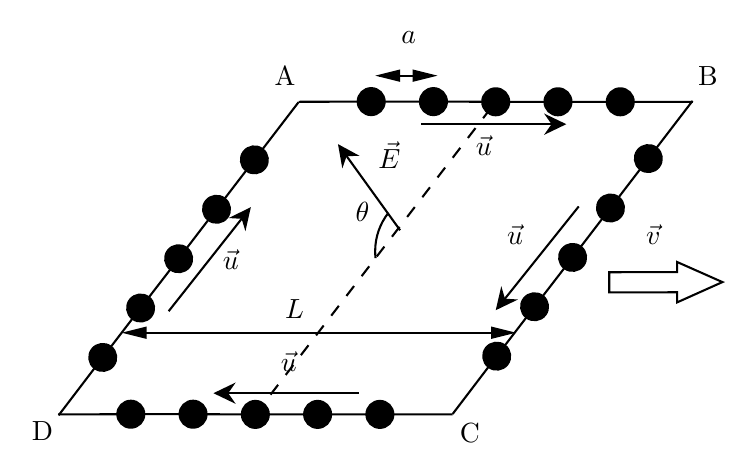
\begin{tikzpicture}[x=0.75pt,y=0.75pt,yscale=-1,xscale=1]
%uncomment if require: \path (0,934); %set diagram left start at 0, and has height of 934

%Straight Lines [id:da8868121237900741] 
\draw    (306,200) -- (239,200) ;
\draw [shift={(236,200)}, rotate = 360] [fill={rgb, 255:red, 0; green, 0; blue, 0 }  ][line width=0.08]  [draw opacity=0] (10.72,-5.15) -- (0,0) -- (10.72,5.15) -- (7.12,0) -- cycle    ;
%Shape: Circle [id:dp024769016873130267] 
\draw  [fill={rgb, 255:red, 0; green, 0; blue, 0 }  ,fill opacity=1 ] (305.5,59.52) .. controls (305.5,55.93) and (308.41,53.02) .. (312,53.02) .. controls (315.59,53.02) and (318.5,55.93) .. (318.5,59.52) .. controls (318.5,63.11) and (315.59,66.02) .. (312,66.02) .. controls (308.41,66.02) and (305.5,63.11) .. (305.5,59.52) -- cycle ;
%Shape: Circle [id:dp35421786023734736] 
\draw  [fill={rgb, 255:red, 0; green, 0; blue, 0 }  ,fill opacity=1 ] (335.5,59.52) .. controls (335.5,55.93) and (338.41,53.02) .. (342,53.02) .. controls (345.59,53.02) and (348.5,55.93) .. (348.5,59.52) .. controls (348.5,63.11) and (345.59,66.02) .. (342,66.02) .. controls (338.41,66.02) and (335.5,63.11) .. (335.5,59.52) -- cycle ;
%Shape: Circle [id:dp8473148960925541] 
\draw  [fill={rgb, 255:red, 0; green, 0; blue, 0 }  ,fill opacity=1 ] (365.5,59.61) .. controls (365.5,56.02) and (368.41,53.11) .. (372,53.11) .. controls (375.59,53.11) and (378.5,56.02) .. (378.5,59.61) .. controls (378.5,63.2) and (375.59,66.11) .. (372,66.11) .. controls (368.41,66.11) and (365.5,63.2) .. (365.5,59.61) -- cycle ;
%Shape: Circle [id:dp8678368760400528] 
\draw  [fill={rgb, 255:red, 0; green, 0; blue, 0 }  ,fill opacity=1 ] (395.5,59.61) .. controls (395.5,56.02) and (398.41,53.11) .. (402,53.11) .. controls (405.59,53.11) and (408.5,56.02) .. (408.5,59.61) .. controls (408.5,63.2) and (405.59,66.11) .. (402,66.11) .. controls (398.41,66.11) and (395.5,63.2) .. (395.5,59.61) -- cycle ;
%Straight Lines [id:da20311584567442176] 
\draw    (277,59.61) -- (312,59.52) -- (342,59.52) -- (372,59.61) -- (402,59.61) -- (432,59.61) -- (467,59.61) ;
%Shape: Circle [id:dp8166102454283666] 
\draw  [fill={rgb, 255:red, 0; green, 0; blue, 0 }  ,fill opacity=1 ] (425.5,59.61) .. controls (425.5,56.02) and (428.41,53.11) .. (432,53.11) .. controls (435.59,53.11) and (438.5,56.02) .. (438.5,59.61) .. controls (438.5,63.2) and (435.59,66.11) .. (432,66.11) .. controls (428.41,66.11) and (425.5,63.2) .. (425.5,59.61) -- cycle ;

%Shape: Circle [id:dp2573354582604783] 
\draw  [fill={rgb, 255:red, 0; green, 0; blue, 0 }  ,fill opacity=1 ] (178.71,187.94) .. controls (175.86,185.75) and (175.32,181.67) .. (177.5,178.82) .. controls (179.69,175.97) and (183.77,175.43) .. (186.62,177.62) .. controls (189.47,179.8) and (190.01,183.88) .. (187.82,186.73) .. controls (185.64,189.58) and (181.56,190.12) .. (178.71,187.94) -- cycle ;
%Shape: Circle [id:dp6794638166583198] 
\draw  [fill={rgb, 255:red, 0; green, 0; blue, 0 }  ,fill opacity=1 ] (196.96,164.12) .. controls (194.11,161.94) and (193.57,157.86) .. (195.75,155.01) .. controls (197.93,152.16) and (202.01,151.62) .. (204.86,153.8) .. controls (207.71,155.99) and (208.25,160.07) .. (206.07,162.92) .. controls (203.89,165.77) and (199.81,166.31) .. (196.96,164.12) -- cycle ;
%Shape: Circle [id:dp8793351711019681] 
\draw  [fill={rgb, 255:red, 0; green, 0; blue, 0 }  ,fill opacity=1 ] (215.27,140.37) .. controls (212.42,138.18) and (211.88,134.1) .. (214.07,131.25) .. controls (216.25,128.4) and (220.33,127.86) .. (223.18,130.05) .. controls (226.03,132.23) and (226.57,136.31) .. (224.39,139.16) .. controls (222.2,142.01) and (218.12,142.55) .. (215.27,140.37) -- cycle ;
%Shape: Circle [id:dp030910884504322222] 
\draw  [fill={rgb, 255:red, 0; green, 0; blue, 0 }  ,fill opacity=1 ] (233.52,116.55) .. controls (230.67,114.37) and (230.13,110.29) .. (232.31,107.44) .. controls (234.5,104.59) and (238.58,104.05) .. (241.43,106.23) .. controls (244.28,108.42) and (244.82,112.5) .. (242.63,115.35) .. controls (240.45,118.2) and (236.37,118.74) .. (233.52,116.55) -- cycle ;
%Straight Lines [id:da6508716644788097] 
\draw    (161.45,210.61) -- (182.66,182.78) -- (200.91,158.96) -- (219.23,135.21) -- (237.47,111.39) -- (255.72,87.58) -- (277.01,59.8) ;
%Shape: Circle [id:dp26654850192896107] 
\draw  [fill={rgb, 255:red, 0; green, 0; blue, 0 }  ,fill opacity=1 ] (251.77,92.74) .. controls (248.92,90.56) and (248.38,86.48) .. (250.56,83.63) .. controls (252.74,80.78) and (256.82,80.24) .. (259.67,82.42) .. controls (262.52,84.6) and (263.06,88.68) .. (260.88,91.53) .. controls (258.7,94.38) and (254.62,94.92) .. (251.77,92.74) -- cycle ;

%Shape: Circle [id:dp6111992447070662] 
\draw  [fill={rgb, 255:red, 0; green, 0; blue, 0 }  ,fill opacity=1 ] (189.69,210.13) .. controls (189.69,206.54) and (192.6,203.63) .. (196.19,203.63) .. controls (199.78,203.63) and (202.69,206.54) .. (202.69,210.13) .. controls (202.69,213.72) and (199.78,216.63) .. (196.19,216.63) .. controls (192.6,216.63) and (189.69,213.72) .. (189.69,210.13) -- cycle ;
%Shape: Circle [id:dp3591779217714379] 
\draw  [fill={rgb, 255:red, 0; green, 0; blue, 0 }  ,fill opacity=1 ] (219.69,210.13) .. controls (219.69,206.54) and (222.6,203.63) .. (226.19,203.63) .. controls (229.78,203.63) and (232.69,206.54) .. (232.69,210.13) .. controls (232.69,213.72) and (229.78,216.63) .. (226.19,216.63) .. controls (222.6,216.63) and (219.69,213.72) .. (219.69,210.13) -- cycle ;
%Shape: Circle [id:dp13672279031874401] 
\draw  [fill={rgb, 255:red, 0; green, 0; blue, 0 }  ,fill opacity=1 ] (249.69,210.22) .. controls (249.69,206.63) and (252.6,203.72) .. (256.19,203.72) .. controls (259.78,203.72) and (262.69,206.63) .. (262.69,210.22) .. controls (262.69,213.81) and (259.78,216.72) .. (256.19,216.72) .. controls (252.6,216.72) and (249.69,213.81) .. (249.69,210.22) -- cycle ;
%Shape: Circle [id:dp4884432582074689] 
\draw  [fill={rgb, 255:red, 0; green, 0; blue, 0 }  ,fill opacity=1 ] (279.69,210.22) .. controls (279.69,206.63) and (282.6,203.72) .. (286.19,203.72) .. controls (289.78,203.72) and (292.69,206.63) .. (292.69,210.22) .. controls (292.69,213.81) and (289.78,216.72) .. (286.19,216.72) .. controls (282.6,216.72) and (279.69,213.81) .. (279.69,210.22) -- cycle ;
%Straight Lines [id:da7590538991419882] 
\draw    (161.19,210.22) -- (196.19,210.13) -- (226.19,210.13) -- (256.19,210.22) -- (286.19,210.22) -- (316.19,210.22) -- (351.19,210.22) ;
%Shape: Circle [id:dp4694752429861433] 
\draw  [fill={rgb, 255:red, 0; green, 0; blue, 0 }  ,fill opacity=1 ] (309.69,210.22) .. controls (309.69,206.63) and (312.6,203.72) .. (316.19,203.72) .. controls (319.78,203.72) and (322.69,206.63) .. (322.69,210.22) .. controls (322.69,213.81) and (319.78,216.72) .. (316.19,216.72) .. controls (312.6,216.72) and (309.69,213.81) .. (309.69,210.22) -- cycle ;

%Shape: Circle [id:dp5503261396577237] 
\draw  [fill={rgb, 255:red, 0; green, 0; blue, 0 }  ,fill opacity=1 ] (368.52,187.32) .. controls (365.67,185.14) and (365.13,181.06) .. (367.31,178.21) .. controls (369.5,175.36) and (373.58,174.82) .. (376.42,177) .. controls (379.27,179.19) and (379.81,183.27) .. (377.63,186.12) .. controls (375.45,188.97) and (371.37,189.51) .. (368.52,187.32) -- cycle ;
%Shape: Circle [id:dp7454866762610632] 
\draw  [fill={rgb, 255:red, 0; green, 0; blue, 0 }  ,fill opacity=1 ] (386.76,163.51) .. controls (383.91,161.33) and (383.37,157.25) .. (385.56,154.4) .. controls (387.74,151.55) and (391.82,151.01) .. (394.67,153.19) .. controls (397.52,155.37) and (398.06,159.45) .. (395.88,162.3) .. controls (393.69,165.15) and (389.61,165.69) .. (386.76,163.51) -- cycle ;
%Shape: Circle [id:dp118030926236806] 
\draw  [fill={rgb, 255:red, 0; green, 0; blue, 0 }  ,fill opacity=1 ] (405.08,139.75) .. controls (402.23,137.57) and (401.69,133.49) .. (403.88,130.64) .. controls (406.06,127.79) and (410.14,127.25) .. (412.99,129.43) .. controls (415.84,131.61) and (416.38,135.69) .. (414.2,138.54) .. controls (412.01,141.39) and (407.93,141.93) .. (405.08,139.75) -- cycle ;
%Shape: Circle [id:dp15819496315151405] 
\draw  [fill={rgb, 255:red, 0; green, 0; blue, 0 }  ,fill opacity=1 ] (423.33,115.94) .. controls (420.48,113.75) and (419.94,109.67) .. (422.12,106.82) .. controls (424.31,103.97) and (428.39,103.43) .. (431.24,105.62) .. controls (434.09,107.8) and (434.63,111.88) .. (432.44,114.73) .. controls (430.26,117.58) and (426.18,118.12) .. (423.33,115.94) -- cycle ;
%Straight Lines [id:da9800576924701969] 
\draw    (351.26,210) -- (372.47,182.16) -- (390.72,158.35) -- (409.04,134.59) -- (427.28,110.78) -- (445.53,86.96) -- (466.82,59.18) ;
%Shape: Circle [id:dp7000349022845087] 
\draw  [fill={rgb, 255:red, 0; green, 0; blue, 0 }  ,fill opacity=1 ] (441.58,92.12) .. controls (438.73,89.94) and (438.19,85.86) .. (440.37,83.01) .. controls (442.55,80.16) and (446.63,79.62) .. (449.48,81.8) .. controls (452.33,83.99) and (452.87,88.07) .. (450.69,90.92) .. controls (448.5,93.77) and (444.42,94.31) .. (441.58,92.12) -- cycle ;

%Straight Lines [id:da8917915430019516] 
\draw    (214.43,160.5) -- (252.15,112.75) ;
\draw [shift={(254.01,110.4)}, rotate = 128.31] [fill={rgb, 255:red, 0; green, 0; blue, 0 }  ][line width=0.08]  [draw opacity=0] (10.72,-5.15) -- (0,0) -- (10.72,5.15) -- (7.12,0) -- cycle    ;
%Straight Lines [id:da0642736528117065] 
\draw  [dash pattern={on 4.5pt off 4.5pt}]  (256.19,210.22) -- (372,59.61) ;
%Straight Lines [id:da09025453177104081] 
\draw    (325.93,121.5) -- (297.75,82.43) ;
\draw [shift={(296,80)}, rotate = 54.2] [fill={rgb, 255:red, 0; green, 0; blue, 0 }  ][line width=0.08]  [draw opacity=0] (10.72,-5.15) -- (0,0) -- (10.72,5.15) -- (7.12,0) -- cycle    ;
%Straight Lines [id:da24076810236908086] 
\draw    (193.79,170.87) -- (379.79,170.87) ;
\draw [shift={(381.79,170.87)}, rotate = 180] [fill={rgb, 255:red, 0; green, 0; blue, 0 }  ][line width=0.08]  [draw opacity=0] (12,-3) -- (0,0) -- (12,3) -- cycle    ;
\draw [shift={(191.79,170.87)}, rotate = 0] [fill={rgb, 255:red, 0; green, 0; blue, 0 }  ][line width=0.08]  [draw opacity=0] (12,-3) -- (0,0) -- (12,3) -- cycle    ;
%Straight Lines [id:da6638185067888682] 
\draw    (412.01,110.02) -- (373.88,157.68) ;
\draw [shift={(372.01,160.02)}, rotate = 308.66] [fill={rgb, 255:red, 0; green, 0; blue, 0 }  ][line width=0.08]  [draw opacity=0] (10.72,-5.15) -- (0,0) -- (10.72,5.15) -- (7.12,0) -- cycle    ;
%Straight Lines [id:da24594238389731293] 
\draw    (336.01,70.4) -- (403.01,70.4) ;
\draw [shift={(406.01,70.4)}, rotate = 180] [fill={rgb, 255:red, 0; green, 0; blue, 0 }  ][line width=0.08]  [draw opacity=0] (10.72,-5.15) -- (0,0) -- (10.72,5.15) -- (7.12,0) -- cycle    ;
%Shape: Arc [id:dp1654755284756213] 
\draw  [draw opacity=0] (314.1,134.92) .. controls (313.98,133.83) and (313.92,132.72) .. (313.92,131.6) .. controls (313.92,124.66) and (316.27,118.27) .. (320.23,113.19) -- (343.92,131.6) -- cycle ; \draw   (314.1,134.92) .. controls (313.98,133.83) and (313.92,132.72) .. (313.92,131.6) .. controls (313.92,124.66) and (316.27,118.27) .. (320.23,113.19) ;
%Down Arrow [id:dp657617897326547] 
\draw   (459.44,156.24) -- (459.43,151.38) -- (426.71,151.45) -- (426.69,141.73) -- (459.41,141.66) -- (459.4,136.8) -- (481.23,146.47) -- cycle ;
%Straight Lines [id:da7479086208396557] 
\draw    (316,47.02) -- (342,47.02) ;
\draw [shift={(344,47.02)}, rotate = 180] [fill={rgb, 255:red, 0; green, 0; blue, 0 }  ][line width=0.08]  [draw opacity=0] (12,-3) -- (0,0) -- (12,3) -- cycle    ;
\draw [shift={(314,47.02)}, rotate = 0] [fill={rgb, 255:red, 0; green, 0; blue, 0 }  ][line width=0.08]  [draw opacity=0] (12,-3) -- (0,0) -- (12,3) -- cycle    ;

% Text Node
\draw (267,178.4) node [anchor=north west][inner sep=0.75pt]    {$\vec{u}$};
% Text Node
\draw (147,212) node [anchor=north west][inner sep=0.75pt]   [align=left] {D};
% Text Node
\draw (376,117.4) node [anchor=north west][inner sep=0.75pt]    {$\vec{u}$};
% Text Node
\draw (303,106.4) node [anchor=north west][inner sep=0.75pt]    {$\theta $};
% Text Node
\draw (314,77.4) node [anchor=north west][inner sep=0.75pt]    {$\vec{E}$};
% Text Node
\draw (264,41) node [anchor=north west][inner sep=0.75pt]   [align=left] {A};
% Text Node
\draw (468,41) node [anchor=north west][inner sep=0.75pt]   [align=left] {B};
% Text Node
\draw (353.26,213) node [anchor=north west][inner sep=0.75pt]   [align=left] {C};
% Text Node
\draw (443,117.4) node [anchor=north west][inner sep=0.75pt]    {$\vec{v}$};
% Text Node
\draw (325,24.4) node [anchor=north west][inner sep=0.75pt]    {$a$};
% Text Node
\draw (239,129.4) node [anchor=north west][inner sep=0.75pt]    {$\vec{u}$};
% Text Node
\draw (361,74.4) node [anchor=north west][inner sep=0.75pt]    {$\vec{u}$};
% Text Node
\draw (269,153.4) node [anchor=north west][inner sep=0.75pt]    {$L$};


\end{tikzpicture}
\end{center}
  Xét tình huống mà khung chuyển động với vận tốc $v$ song song với cạnh ${AB}$ (hình vẽ) trong một điện trường đều có cường độ $\ot{E}$ hướng vuông góc với vận tốc của khung và tạo một góc $\theta$ so với mặt phẳng của khung.\\
Xét cả các hiệu ứng tương đối tính, hãy tính độ lớn các đại lượng sau trong hệ quy chiếu của quan sát viên nhìn thấy khung chuyển động với vận tốc $v$:
\begin{enumerate}[1)]
    \item Khoảng cách giữa các quả bóng trên các cạnh $a_{A B}, a_{B C}, a_{C D}$, và $a_{D A}$.
\item Tổng điện tích của cạnh khung dây và các quả cầu trên mỗi cạnh $Q_{A B}, Q_{B C}, Q_{C D}$ và $Q_{D A}$.
\item Độ lớn của moment lực $M$ mà điện trường cố gắng quay hệ khung dây cùng các quả cầu.
\item Năng lượng tương tác $W$ của hệ bao gồm khung và các quả cầu với điện trường. Tất cả các câu trả lời phải biểu diễn qua các đại lượng cho ở đề bài. Điện tích của một vật cô lập không phụ thuộc vào hệ quy chiếu mà ta đo nó. Tất cả các hiệu ứng bức xạ sóng điện từ được bỏ qua.
\end{enumerate}
\end{vd}
\begin{loigiai}
\begin{enumerate}[1)]
    \item Gọi $S$ là hệ quy chiếu phòng thí nghiệm (người quan sát), $S$ thấy khung dây chuyển động với vận tốc $v$; $S'$ là hệ quy chiếu khung dây (trục $x’$ của hệ này sẽ được lấy cùng hướng với $v$, $y'$ theo phương của cạnh $DA$ và trục $z’$ vuông góc với mặt phẳng của khung). Các trục của $S$ song song với trục của $S’$ và gốc tọa độ của cả hai hệ trùng nhau tại $t = 0$.
\begin{enumerate}[a)]
    \item Cạnh $AB$:\\
    $S_{AB}$ là hệ quy chiếu tại đó các quả cầu chuyển động trong khi cạnh $AB$ đứng yên. Các trục của nó song song với trục của $S$ và $S'$. $S''$ có vận tốc $u$ so với $S'$.\\
    Theo sự co Lorentz, khoảng cách $a$, giữa các quả cầu liền kề của $AB$, trong hệ quy chiếu $S''$ là:
    \[a_{r}=\dfrac{a}{\sqrt{1-\dfrac{u^{2}}{c^{2}}}}. \tag{1} \label{humeo1}\]
    (Kết quả này có giá trị đối với khoảng cách giữa hai quả bóng liền kề bất kỳ nếu $a$ được đo trong hệ quy chiếu mà chúng ở trạng thái nghỉ.)\\
    Do tính cộng tương đối của các vận tốc, một người quan sát ở $S$ thấy các quả cầu chuyển động trên $AB$ với vận tốc:
    \[u_{A B}=\dfrac{v+u}{1+\dfrac{u v}{c^{2}}}. \tag{2} \label{humeo2}\]
    Vì vậy, do sự co Lorentz, người quan sát này sẽ thấy khoảng cách giữa các quả cầu như sau: 
    \[a_{A B}=\sqrt{1-\dfrac{u_{A B}^{2}}{c^{2}}} a_{r}. \tag{3} \label{humeo3}\]
    Từ (\ref{humeo1}), (\ref{humeo2}), (\ref{humeo3}), ta thu được:
    \[a_{A B}=\sqrt{\dfrac{1-\dfrac{v^{2}}{t^{2}}}{1+\dfrac{u v}{c^{2}}}} a. \tag{4} \label{humeo4}\]
    \item Cạnh $CD:$\\
    Đối với người quan sát $S$, vận tốc quả cầu ở cạnh $CD$ là:
    \[u_{C D}=\dfrac{v-u}{1-\dfrac{u v}{c^{2}}}. \tag{5} \label{humeo5}\]
    Theo sự co Lorentz:
    \[a_{C D}=\sqrt{1-\dfrac{u_{C D}^{2}}{c^{2}}} a_{r}. \tag{6} \label{humeo6}\]
    Từ (\ref{humeo1}), (\ref{humeo5}), (\ref{humeo6}), ta được:
    \[a_{C D}=\dfrac{\sqrt{1-\dfrac{v^{2}}{c^{2}}}}{1-\dfrac{u v}{c^{2}}} a. \tag{7}\]
    \item Cạnh $DA$:\\
    Trong hệ quy chiếu $S'$, tại thời điểm $t_0'$, gọi một quả cầu có tọa độ là $x_1' = y_1' = z_1' = 0$, cùng thời điểm đó, quả cầu kế tiếp nó sẽ nằm ở vị trí $x_{2}^{\prime}=0, y_{2}^{\prime}=a, z_{2}^{\prime}=0$.\\
    Dùng công thức biến đổi Lorentz, ta có:
\[\heva{x&=\dfrac{1}{\sqrt{1-\dfrac{v^{2}}{c^{2}}}}\left(x^{\prime}+v t^{\prime}\right),\\
y&=y',\\
z&=z',\\
t&=\dfrac{1}{\sqrt{1-\dfrac{v^{2}}{c^{2}}}}\left(t^{\prime}+\dfrac{x^{\prime} v}{c^{2}}\right).} \tag{8}\]
Theo đó, chúng ta có quả cầu đầu tiên trong hệ quy chiếu $S$:
\[
x_{1}=\dfrac{1}{\sqrt{1-\dfrac{v^{2}}{c^{2}}}} v t_{o}^{\prime} ;\ {y}_{1}=0 ;\ {z}_{1}=0 ;\ {t}_{1}=\dfrac{1}{\sqrt{1-\dfrac{{v}^{2}}{{c}^{2}}}} {t}_{0}^{\prime}. \tag{9}
\]
Và thứ hai:
\[
x_{2}=\dfrac{1}{\sqrt{1-\dfrac{v^{2}}{c^{2}}}} v t_{0}^{\prime} ;\ y_{2}=a ;\ z_{2}=0 ;\ t_{2}=\dfrac{1}{\sqrt{1-\dfrac{v^{2}}{c^{2}}}} t_{0}^{\prime}. \tag{10}
\]
Tại $t_1=t_2$, khoảng cách giữa các bóng được cho bởi:
\[
a_{D A}=\left(x_{2}-x_{1}\right)^{2}+\left(y_{2}-y_{1}\right)^{2}+\left(z_{2}-z_{1}\right)^{2}. \tag{11}
\]
Và vì vậy:
\[a_{DA}=a. \tag{12}\]
\item Cạnh $BC$:\\
Chúng ta làm tương tự như cạnh $DA$ và dễ dàng chứng minh được rằng:
\[a_{BC}=a.\tag{13}\]
\end{enumerate}
\item Điện tích của dây trên bất kỳ cạnh nào, trong hệ quy chiếu liên kết với vòng dây có thể được tính như sau:
\[
{Q}_\text{{dây}}=-\dfrac{{L}}{{a}} {q}. \tag{14} \label{humeo14}
\]
Vì $L/a$ chính là số quả cầu ở mặt đó. Do điện tích bất biến, nên có thể đo cùng một điện tích ở mỗi bên của dây dẫn trong hệ quy chiếu phòng thí nghiệm (quan sát viên).
\begin{enumerate}[a)]
    \item Cạnh $AB$:\\
    Điện tích tương ứng với các quả cầu trong cạnh $AB$, trong hệ quy chiếu phòng thí nghiệm là:
    \[
Q_{\text{cầu }AB}=\dfrac{Lq \sqrt{1-\dfrac{v^{2}}{c^{2}}}}{a_{A B}}. \tag{15} \label{humeo15}
\]
Điều này có được từ phép nhân số lượng quả cầu trong cạnh đó với điện tích (bất biến) của một quả cầu. Thừa số đầu tiên của tử số ở vế phải của phương trình (\ref{humeo15}) là khoảng cách quy ước mà người quan sát đo được và mẫu số là khoảng cách giữa các quả cầu trong cạnh đó. Thay vào (\ref{humeo15}) phương trình (\ref{humeo4}), ta được:
\[
{Q}_{\text{cầu }AB}=\left(\dfrac{1+{u v}}{{c}^{2}}\right) \dfrac{{Lq}}{{a}}. \tag{16} \label{humeo16}
\]
Cộng (\ref{humeo14}) và (\ref{humeo16}), ta tính được điện tích tổng cộng trên cạnh $AB$:
\[
{Q}_{{AB}}=\dfrac{{uv}}{{c}^{2}} \dfrac{{L}}{{a}} {q}. \tag{17} \label{humeo17}
\]
\item Cạnh $CD$:
Tương tự như trên, ta cũng có:
\[{Q}_{\text{cầu }CD}=\left(\dfrac{1-{u v}}{{c}^{2}}\right) \dfrac{{Lq}}{{a}}. \tag{18} \label{humeo18}\]
Cộng (\ref{humeo14}) và (\ref{humeo18}), ta thu được:
\[
{Q}_{{CD}}=-\frac{{uv}}{{c}^{2}} \frac{{L}}{{a}} {q}. \label{19}
\]
Độ dài của các cạnh này mà người quan sát đo được trong $S$ là $L$ và khoảng cách giữa các quả bóng là $a$, do đó:
\[Q_{\text{cầu }CD}=Q_{\text{cầu }DA}=\dfrac{qL}{a}.\tag{20} \label{humeo20}\]
Cộng phương trình (\ref{humeo14} và (\ref{humeo20}) ta được:
\[Q_{BC}=0. \tag{21.1}\]
\[Q_{DA}=0. \tag{21.2}\]

\end{enumerate}
\item Lực điện tác dụng lên cạnh $AB$ là;
\[
\overrightarrow{{F}_{{AB}}}={Q}_{{AB}} \overrightarrow{{E}}=\left(\dfrac{{uv}}{{c}^{2}}\right) \dfrac{{L}}{{a}} {q} \overrightarrow{{E}}.\tag{22}
\]
Lực điện tác dụng lên cạnh $CD$ là:
\[\overrightarrow{{F}_{{CD}}}={Q}_{{CD}} \overrightarrow{{E}}=-\left(\dfrac{{uv}}{{c}^{2}}\right) \dfrac{{L}}{{a}} {q} \overrightarrow{{E}}.\tag{23}\]
\begin{center}

\tikzset{every picture/.style={line width=0.75pt}} %set default line width to 0.75pt        

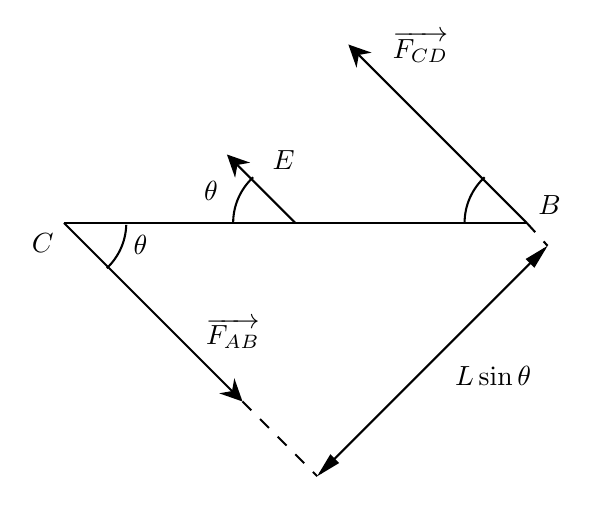
\begin{tikzpicture}[x=0.75pt,y=0.75pt,yscale=-1,xscale=1]
%uncomment if require: \path (0,300); %set diagram left start at 0, and has height of 300

%Straight Lines [id:da584155228361827] 
\draw    (100,117) -- (323,117) ;
%Straight Lines [id:da25520722446728406] 
\draw    (100,117) -- (183.88,200.88) ;
\draw [shift={(186,203)}, rotate = 225] [fill={rgb, 255:red, 0; green, 0; blue, 0 }  ][line width=0.08]  [draw opacity=0] (10.72,-5.15) -- (0,0) -- (10.72,5.15) -- (7.12,0) -- cycle    ;
%Straight Lines [id:da3504238635794259] 
\draw    (323,117) -- (239.12,33.12) ;
\draw [shift={(237,31)}, rotate = 405] [fill={rgb, 255:red, 0; green, 0; blue, 0 }  ][line width=0.08]  [draw opacity=0] (10.72,-5.15) -- (0,0) -- (10.72,5.15) -- (7.12,0) -- cycle    ;
%Straight Lines [id:da5792858866993564] 
\draw    (211.5,117) -- (180.62,86.12) ;
\draw [shift={(178.5,84)}, rotate = 405] [fill={rgb, 255:red, 0; green, 0; blue, 0 }  ][line width=0.08]  [draw opacity=0] (10.72,-5.15) -- (0,0) -- (10.72,5.15) -- (7.12,0) -- cycle    ;
%Straight Lines [id:da0035845008621042673] 
\draw  [dash pattern={on 4.5pt off 4.5pt}]  (323,117) -- (333,128) ;
%Straight Lines [id:da25511610162893916] 
\draw  [dash pattern={on 4.5pt off 4.5pt}]  (186,203) -- (222,239) ;
%Straight Lines [id:da49760269025300263] 
\draw    (223.41,237.59) -- (331.59,129.41) ;
\draw [shift={(333,128)}, rotate = 495] [fill={rgb, 255:red, 0; green, 0; blue, 0 }  ][line width=0.08]  [draw opacity=0] (12,-3) -- (0,0) -- (12,3) -- cycle    ;
\draw [shift={(222,239)}, rotate = 315] [fill={rgb, 255:red, 0; green, 0; blue, 0 }  ][line width=0.08]  [draw opacity=0] (12,-3) -- (0,0) -- (12,3) -- cycle    ;
%Shape: Arc [id:dp6104904383496845] 
\draw  [draw opacity=0] (181.5,117) .. controls (181.5,108.3) and (185.21,100.46) .. (191.13,94.98) -- (211.5,117) -- cycle ; \draw   (181.5,117) .. controls (181.5,108.3) and (185.21,100.46) .. (191.13,94.98) ;
%Shape: Arc [id:dp7057388547061749] 
\draw  [draw opacity=0] (129.99,117.91) .. controls (129.74,126.14) and (126.18,133.54) .. (120.6,138.81) -- (100,117) -- cycle ; \draw   (129.99,117.91) .. controls (129.74,126.14) and (126.18,133.54) .. (120.6,138.81) ;
%Shape: Arc [id:dp982451889847471] 
\draw  [draw opacity=0] (293,117) .. controls (293,108.3) and (296.71,100.46) .. (302.63,94.98) -- (323,117) -- cycle ; \draw   (293,117) .. controls (293,108.3) and (296.71,100.46) .. (302.63,94.98) ;

% Text Node
\draw (287,184.4) node [anchor=north west][inner sep=0.75pt]    {$L\sin \theta $};
% Text Node
\draw (167,161.4) node [anchor=north west][inner sep=0.75pt]    {$\overrightarrow{F_{AB}}$};
% Text Node
\draw (257,23.4) node [anchor=north west][inner sep=0.75pt]    {$\overrightarrow{F_{CD}}$};
% Text Node
\draw (199,80.4) node [anchor=north west][inner sep=0.75pt]    {$\ot{E}$};
% Text Node
\draw (166,95.4) node [anchor=north west][inner sep=0.75pt]    {$\theta $};
% Text Node
\draw (131.99,121.31) node [anchor=north west][inner sep=0.75pt]    {$\theta $};
% Text Node
\draw (83,120.4) node [anchor=north west][inner sep=0.75pt]    {$C$};
% Text Node
\draw (327,102.4) node [anchor=north west][inner sep=0.75pt]    {$B$};


\end{tikzpicture}
\end{center}
$F_{CD}$ và $F_{AB}$ tạo thành một cặp lực. Vì vậy, từ biểu thức moment cho một cặp lực, chúng ta có:
\[
{M}=\left|\overrightarrow{{F}_{{AB}}}\right| {L} \sin \theta. \tag{24}
\]
Và cuối cùng:
\[
{M} = \dfrac{{uv}}{{c}^{2}} \dfrac{{L}^{2}}{{a}}|q| \abs{\overrightarrow{{E}}} \sin \theta. \tag{25}
\]
\item Gọi $V_{AB}$ và $V_{CD}$ lần lượt là điện thế tại các cạnh $AB$ và $CD$. Khi đó: 
\[{W}={V}_{{AB}} {Q}_{{AB}}+{V}_{{CD}} {Q}_{{CD}}. \tag{26}
\]
Điện thế bằng không ($V = 0$) trong mặt phẳng vuông góc với $E$ và cách cạnh $AB$ một khoảng tùy ý (xem hình dưới).
\begin{center}
\tikzset{every picture/.style={line width=0.75pt}} %set default line width to 0.75pt        

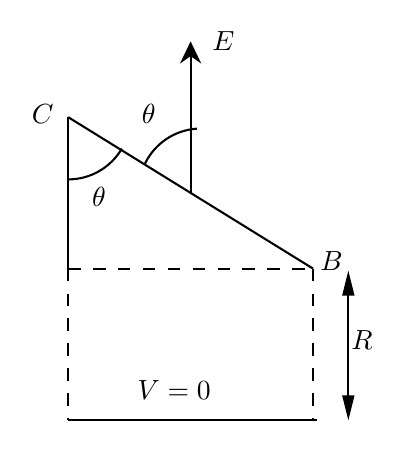
\begin{tikzpicture}[x=0.75pt,y=0.75pt,yscale=-1,xscale=1]
%uncomment if require: \path (0,300); %set diagram left start at 0, and has height of 300

%Straight Lines [id:da6252945047254344] 
\draw    (141,80) -- (259,153) ;
%Straight Lines [id:da4779629107908181] 
\draw    (141,80) -- (141,153) ;
%Straight Lines [id:da4742824307194009] 
\draw  [dash pattern={on 4.5pt off 4.5pt}]  (141,153) -- (259,153) ;
%Straight Lines [id:da7954830651582125] 
\draw    (141,226) -- (261,226) ;
%Straight Lines [id:da941645957868803] 
\draw  [dash pattern={on 4.5pt off 4.5pt}]  (141,153) -- (141,226) ;
%Straight Lines [id:da8803365313984062] 
\draw  [dash pattern={on 4.5pt off 4.5pt}]  (259,153) -- (259,226) ;
%Straight Lines [id:da11141132583313329] 
\draw    (276,156) -- (276,224) ;
\draw [shift={(276,226)}, rotate = 270] [fill={rgb, 255:red, 0; green, 0; blue, 0 }  ][line width=0.08]  [draw opacity=0] (12,-3) -- (0,0) -- (12,3) -- cycle    ;
\draw [shift={(276,154)}, rotate = 90] [fill={rgb, 255:red, 0; green, 0; blue, 0 }  ][line width=0.08]  [draw opacity=0] (12,-3) -- (0,0) -- (12,3) -- cycle    ;
%Shape: Arc [id:dp02639079451616433] 
\draw  [draw opacity=0] (166.88,95.17) .. controls (161.67,104.05) and (152.03,110) .. (141,110) -- (141,80) -- cycle ; \draw   (166.88,95.17) .. controls (161.67,104.05) and (152.03,110) .. (141,110) ;
%Straight Lines [id:da41676375832746015] 
\draw    (200,46.5) -- (200,116.5) ;
\draw [shift={(200,43.5)}, rotate = 90] [fill={rgb, 255:red, 0; green, 0; blue, 0 }  ][line width=0.08]  [draw opacity=0] (10.72,-5.15) -- (0,0) -- (10.72,5.15) -- (7.12,0) -- cycle    ;
%Shape: Arc [id:dp41505813310085404] 
\draw  [draw opacity=0] (178.03,102.35) .. controls (182.63,92.93) and (192.02,86.27) .. (203.04,85.56) -- (205,115.5) -- cycle ; \draw   (178.03,102.35) .. controls (182.63,92.93) and (192.02,86.27) .. (203.04,85.56) ;

% Text Node
\draw (122,72.4) node [anchor=north west][inner sep=0.75pt]    {$C$};
% Text Node
\draw (261,143.4) node [anchor=north west][inner sep=0.75pt]    {$B$};
% Text Node
\draw (173,205.4) node [anchor=north west][inner sep=0.75pt]    {$V=0$};
% Text Node
\draw (276,181.4) node [anchor=north west][inner sep=0.75pt]    {$R$};
% Text Node
\draw (151,112.4) node [anchor=north west][inner sep=0.75pt]    {$\theta $};
% Text Node
\draw (175,72.4) node [anchor=north west][inner sep=0.75pt]    {$\theta $};
% Text Node
\draw (209,37.4) node [anchor=north west][inner sep=0.75pt]    {$\ot{E}$};


\end{tikzpicture}
\end{center}
Từ đó:
\[{W}=-{ERQ}_{{AB}}-{E}({R}+{L} \cos \theta) {Q}_{CD}. \tag{27}\]
Nhưng $Q_{CD}=-Q_{AB}$, vì vậy:
\[{W}=-{ELQ}_{{AB}} \cos \theta. \tag{28} \label{humeo28}\]
Từ (\ref{humeo17}) và (\ref{humeo28}), ta thu được:
\[{W}=\frac{{uvL}^{2} {q} {E}}{{c}^{2} {a}} \cos \theta. \tag{29}\]
\end{enumerate}
\end{loigiai}



